% !TeX program = pdflatex
% Informe editable. Compilar desde la raíz del repositorio con make pdf.
\documentclass[11pt,a4paper]{article}
\pdfminorversion=7
\usepackage[T1]{fontenc}
\usepackage[utf8]{inputenc}
\IfFileExists{spanish.ldf}{\usepackage[spanish,es-tabla]{babel}}{\usepackage[english]{babel}\babelprovide[main,import]{spanish}}
\usepackage{lmodern,microtype}
\usepackage[a4paper,top=25mm,bottom=25mm,left=25mm,right=25mm,headheight=14pt]{geometry}
\usepackage{graphicx,xcolor,booktabs,tabularx,longtable,array}
\input{figuras_conceptuales.tex}
\usepackage{amsmath,amssymb,xfp}
\usepackage{tikz}
\usetikzlibrary{arrows.meta,positioning,calc,fit,babel}
\usepackage{titlesec,fancyhdr,enumitem,caption,float,placeins,needspace,pdflscape,multicol,tocloft}
\usepackage{listings,xurl}
\usepackage[unicode,hidelinks]{hyperref}
\definecolor{acento}{HTML}{284B4F}
\definecolor{gris}{HTML}{555555}
\definecolor{suave}{HTML}{F3F5F5}
\hypersetup{pdftitle={Lumina Retail: El retail que ve, decide y actúa en tiempo real},pdfauthor={RetailSmart Global},pdflang={es-PE},bookmarksnumbered=true}
\input{parametros.tex}
\graphicspath{{../report-resources/figures/portadas/}{../report-resources/figures/vinetas/}{../report-resources/figures/apoyo/}{../report-resources/figures/arquitectura/}}
\newcolumntype{Y}{>{\raggedright\arraybackslash}X}
\newcolumntype{P}[1]{>{\raggedright\arraybackslash}p{#1}}
\setlength{\parindent}{0pt}
\setlength{\parskip}{5pt plus 1pt}
\setlength{\emergencystretch}{3em}
\raggedbottom
\setlength{\tabcolsep}{5pt}
\renewcommand{\arraystretch}{1.18}
\linespread{1.06}
\setlist[itemize]{nosep,leftmargin=1.4em,topsep=3pt}
\setlist[enumerate]{nosep,leftmargin=1.6em,topsep=3pt}
\captionsetup{font=small,labelfont=bf,skip=6pt}
\captionsetup[table]{position=top}
\titleformat{\section}{\Large\bfseries}{\thesection}{.7em}{}
\titleformat{\subsection}{\normalsize\bfseries}{\thesubsection}{.65em}{}
\titlespacing*{\section}{0pt}{17pt}{8pt}
\titlespacing*{\subsection}{0pt}{11pt}{4pt}
\pagestyle{fancy}
\fancyhf{}
\fancyhead[L]{\small\textsc{Lumina Retail}}
\fancyhead[R]{\small Arquitectura de datos}
\fancyfoot[C]{\small\thepage}
\renewcommand{\headrulewidth}{.3pt}
\renewcommand{\footrulewidth}{0pt}
\renewcommand{\contentsname}{Índice general}
\renewcommand{\listfigurename}{Índice de figuras}
\renewcommand{\listtablename}{Índice de tablas}
\renewcommand{\figurename}{Figura}
\renewcommand{\tablename}{Tabla}
\renewcommand{\refname}{Fuentes técnicas y de datos}
% Babel fija estos títulos al iniciar el documento: se redefinen después.
\AtBeginDocument{%
  \renewcommand{\contentsname}{Índice general}%
  \renewcommand{\listfigurename}{Índice de figuras}%
  \renewcommand{\listtablename}{Índice de tablas}%
  \renewcommand{\tablename}{Tabla}%
  \renewcommand{\refname}{Fuentes técnicas y de datos}%
}
\clubpenalty=10000
\widowpenalty=10000
\setcounter{tocdepth}{2}
\setcounter{secnumdepth}{2}
\setlength{\cftsecnumwidth}{3em}
\setlength{\cftsubsecnumwidth}{4em}
\newcommand{\Fuente}[1]{{\footnotesize\textit{Fuente: #1.}}}
\newcommand{\ID}[1]{\texttt{#1}}
\newcommand{\Seccion}[1]{\FloatBarrier\Needspace{5\baselineskip}\section{#1}}
\newcommand{\AperturaCapitulo}[3]{%
  \clearpage
  \FloatBarrier
  \refstepcounter{section}%
  \label{#3}%
  \sectionmark{#1}%
  \addcontentsline{toc}{section}{\protect\numberline{\thesection}#1}%
  \thispagestyle{empty}%
  \begin{center}
    \vspace*{.07\textheight}
    \rule{.86\linewidth}{.7pt}\par
    \vspace{7mm}
    {\fontsize{12}{14}\selectfont\textsc{Capítulo}\par}
    \vspace{2mm}
    {\fontsize{40}{44}\selectfont\bfseries\thesection\par}
    \vspace{4mm}
    \parbox{.90\linewidth}{\centering\fontsize{24}{29}\selectfont\bfseries #1\par}
    \vspace{5mm}
    \rule{.86\linewidth}{.7pt}\par
    \vspace{8mm}
    \includegraphics[width=.72\linewidth,height=.38\textheight,keepaspectratio]{#2}
  \end{center}
  \clearpage
}
\newcommand{\AperturaAnexos}[1]{%
  \clearpage
  \phantomsection\addcontentsline{toc}{section}{Anexos}%
  \thispagestyle{empty}%
  \begin{center}
    \vspace*{.15\textheight}
    \rule{.86\linewidth}{.7pt}\par
    \vspace{7mm}
    {\fontsize{12}{14}\selectfont\textsc{Anexos}\par}
    \vspace{5mm}
    \rule{.86\linewidth}{.7pt}\par
    \vspace{10mm}
    \includegraphics[width=.72\linewidth,height=.38\textheight,keepaspectratio]{#1}
  \end{center}
  \clearpage
}
\newcommand{\GraficoApoyo}[4][.78\linewidth]{%
  \begin{figure}[!htbp]
    \centering
    \includegraphics[width=#1,keepaspectratio]{#2.pdf}
    \caption{#3}\label{#4}
    \Fuente{Síntesis visual del contenido del informe y del diseño aprobado}
  \end{figure}
}
\newcommand{\GraficoApoyoDenso}[3]{%
  \GraficoApoyo[.94\linewidth]{#1}{#2}{#3}%
}
\newcommand{\Vinetta}[2]{%
  \par\noindent
  \begin{minipage}[t]{.76\linewidth}
    \vspace{0pt}#2\par
  \end{minipage}\hfill
  \begin{minipage}[t]{.20\linewidth}
    \vspace{0pt}\centering
    \includegraphics[width=2.05cm,height=2.05cm,keepaspectratio]{#1}
  \end{minipage}\par
}
\makeatletter
\newcommand{\LuminaDetalleBegin}{%
  \clearpage
  \FloatBarrier
  \newgeometry{margin=10mm}%
  \paperwidth=297mm
  \paperheight=210mm
  \pdfpagewidth=\paperwidth
  \pdfpageheight=\paperheight
  \textwidth=277mm
  \textheight=190mm
  \hsize=\textwidth
  \linewidth=\textwidth
  \columnwidth=\textwidth
  \@colht=\textheight
  \@colroom=\textheight
  \vsize=\textheight
}
\newcommand{\LuminaDetalleRestore}{%
  \clearpage
  \paperwidth=210mm
  \paperheight=297mm
  \pdfpagewidth=\paperwidth
  \pdfpageheight=\paperheight
  \restoregeometry
  \hsize=\textwidth
  \linewidth=\textwidth
  \columnwidth=\textwidth
  \@colht=\textheight
  \@colroom=\textheight
  \vsize=\textheight
}
\makeatother
\lstset{basicstyle=\ttfamily\footnotesize,breaklines=true,frame=single,rulecolor=\color{black!25},columns=fullflexible,keepspaces=true,showstringspaces=false,aboveskip=7pt,belowskip=7pt}

\begin{document}
\hypersetup{pageanchor=false}
\begin{titlepage}
\centering
\vspace*{18mm}
{\fontsize{40}{46}\selectfont\bfseries Lumina Retail\par}
\vspace{9mm}
{\fontsize{20}{31}\selectfont\bfseries
Datos conectados.\\[2mm]
Operación sincronizada.\par}
\vspace{7mm}
{\color{acento}\rule{35mm}{.7pt}\par}
\vspace{7mm}
{\fontsize{16}{20}\selectfont
Anticipar la demanda. Optimizar el inventario.\\
Acelerar la entrega.\par}
\vspace{2mm}
\resizebox{1\textwidth}{!}{\LuminaPortada}
\vfill
{\normalsize RetailSmart Global\\2026\par}
\vspace*{8mm}
\end{titlepage}

\pagenumbering{roman}
\hypersetup{pageanchor=true}
\clearpage
\begingroup
\footnotesize
\setlength{\parskip}{0pt}
\linespread{1}\selectfont
\tableofcontents
\endgroup
\clearpage
\begingroup
\small
\setlength{\parskip}{0pt}
\linespread{1}\selectfont
\listoffigures
\medskip
\listoftables
\endgroup
\clearpage
\pagenumbering{arabic}

% ================================================================
\AperturaCapitulo{Resumen ejecutivo}{01_resumen_ejecutivo.png}{sec:resumen}
\subsection{Problema de negocio y consecuencias operativas}
RetailSmart Global opera con tiendas físicas y canales de e-commerce sobre una red amplia de tiendas y almacenes. El problema no es únicamente disponer de stock o vender por distintos canales, sino anticipar dónde y cuándo puede agotarse el inventario, si dicho inventario está cerca de la demanda, cuándo la capacidad operativa puede saturarse, cómo se comporta el cliente entre unidades y canales y qué activos pueden degradarse antes de afectar la operación.

Estas brechas se manifiestan en mayores costos de última milla, retrasos durante campañas de alta demanda, quiebres de inventario, decisiones aisladas entre unidades y mantenimiento reactivo. La plataforma no pretende corregir fallas transaccionales del ERP, OMS, WMS, TMS, CRM o sistemas de mantenimiento, sino reducir la demora entre la generación de datos y la toma de decisiones.

\subsection{Solución propuesta y alcance inicial}
Proponemos la Plataforma de Datos RetailSmart como soporte de Lumina Retail, entendida como una capa inteligente de datos que integra información de ventas, pedidos, inventario, logística, clientes, interacción digital y telemetría. Lumina conserva histórico, combina señales recientes y genera alertas, análisis, predicciones y recomendaciones para apoyar a los responsables operacionales.

El principio rector es: \textbf{Lumina observa, integra, analiza, aprende, predice y recomienda; el ecosistema operacional decide y ejecuta}. Por tanto, la solución no sustituye la reserva transaccional de stock, el procesamiento del pedido, el picking, el despacho, el pago, la identidad maestra del cliente ni el mantenimiento físico de activos.

\subsection{Beneficios esperados y decisiones de arquitectura}
El beneficio depende de convertir datos fragmentados en inteligencia accionable. Una señal de caída acelerada de stock puede activar una revisión de reposición; una predicción geográfica puede sustentar el reposicionamiento de inventario; una alerta de saturación puede permitir preparar capacidad; una vista analítica de cliente puede mejorar la comprensión omnicanal; y una anomalía de telemetría puede priorizar una inspección preventiva.

Las decisiones principales son integrar mediante claves gobernadas, combinar streaming, batch, analítica y capacidades predictivas según la pregunta de negocio, separar Bronze, Silver y Gold, preservar la autoridad de los sistemas operacionales y utilizar servicios gestionados de GCP con una excepción explícita frente a la preferencia por código abierto. El avance se condiciona a datos conciliados, responsables de actuación y evidencia medible de valor.


% ================================================================
\AperturaCapitulo{Contexto empresarial y diagnóstico}{02_contexto_diagnostico.png}{sec:contexto}
\subsection{RetailSmart Global y la iniciativa Lumina Retail}
El contexto de negocio de RetailSmart comprende más de nueve millones de clientes activos, ocho regiones logísticas y doce unidades de negocio. La iniciativa Unifica-Retail establece Lumina Retail para aprovechar conjuntamente canales, inventario y activos de distribución. Conviven compras físicas que requieren asistencia y compras móviles que demandan rapidez; ambas necesitan información confiable y oportuna para anticipar demanda, disponibilidad y capacidad.

La lectura adoptada para este informe distingue la visión empresarial completa de RetailSmart de la responsabilidad específica de la plataforma de datos. Lumina no se considera un nuevo núcleo transaccional, sino una capacidad transversal de inteligencia que consume datos del ecosistema operativo y devuelve señales, análisis, predicciones y recomendaciones.

\subsection{Supuestos y frontera funcional de Lumina}
Se asume que RetailSmart dispone, o debe disponer, de sistemas operacionales responsables de pedidos, inventario, reservas, preparación, despacho, entrega, pagos, logística, clientes y mantenimiento. Dichos sistemas continúan siendo la autoridad transaccional y una venta debe poder completarse aunque Lumina esté temporalmente indisponible.

El sistema operacional de inventario es la fuente de verdad del stock actual y de las reservas. De igual forma, se recomienda una capacidad empresarial de Master Data Management (MDM) para resolver identidad canónica, duplicados y atributos maestros de cliente. Lumina consume estas fuentes para análisis, pero no sustituye sus responsabilidades.

\begin{quote}
\textbf{Lumina ayuda a decidir mejor qué hacer; los sistemas operacionales realizan la acción.}
\end{quote}

\subsection{Visión de Lumina Retail}
La visión se interpreta como la construcción de una capa inteligente de datos que conecta analíticamente demanda, inventario, capacidad logística, comportamiento del cliente y condición de activos. Lumina puede identificar desde qué ubicación resulta más conveniente atender una demanda, detectar oportunidades de agrupación o priorización, comparar alternativas de atención y anticipar riesgos de quiebre, saturación o degradación.

Las funcionalidades de reserva de inventario, ejecución de picking, asignación de transporte, seguimiento transaccional del pedido y procesamiento del pago permanecen en los sistemas operacionales. En consecuencia, la compra bajo demanda, la optimización de pedidos y la omnicanalidad se consideran experiencias de negocio habilitadas por inteligencia de Lumina, no acciones ejecutadas directamente por la plataforma.

\subsection{Operación actual y proceso de extremo a extremo}
El proceso comprende captura de demanda, validación de inventario, preparación, despacho, entrega y seguimiento operativo. Los canales, el sistema de pedidos, el ERP, los sistemas de almacén y la logística ejecutan esas actividades. Lumina se ubica fuera de la ruta transaccional obligatoria: recibe datos y eventos de la operación, los integra y produce inteligencia que puede ser consumida por los responsables y aplicaciones correspondientes.

La información parcial entre etapas y los reportes diferidos limitan hoy la capacidad de anticipar problemas. La figura~\ref{fig:proceso-asis} ubica estas limitaciones en el recorrido del pedido.
\begin{figure}[!htbp]
\centering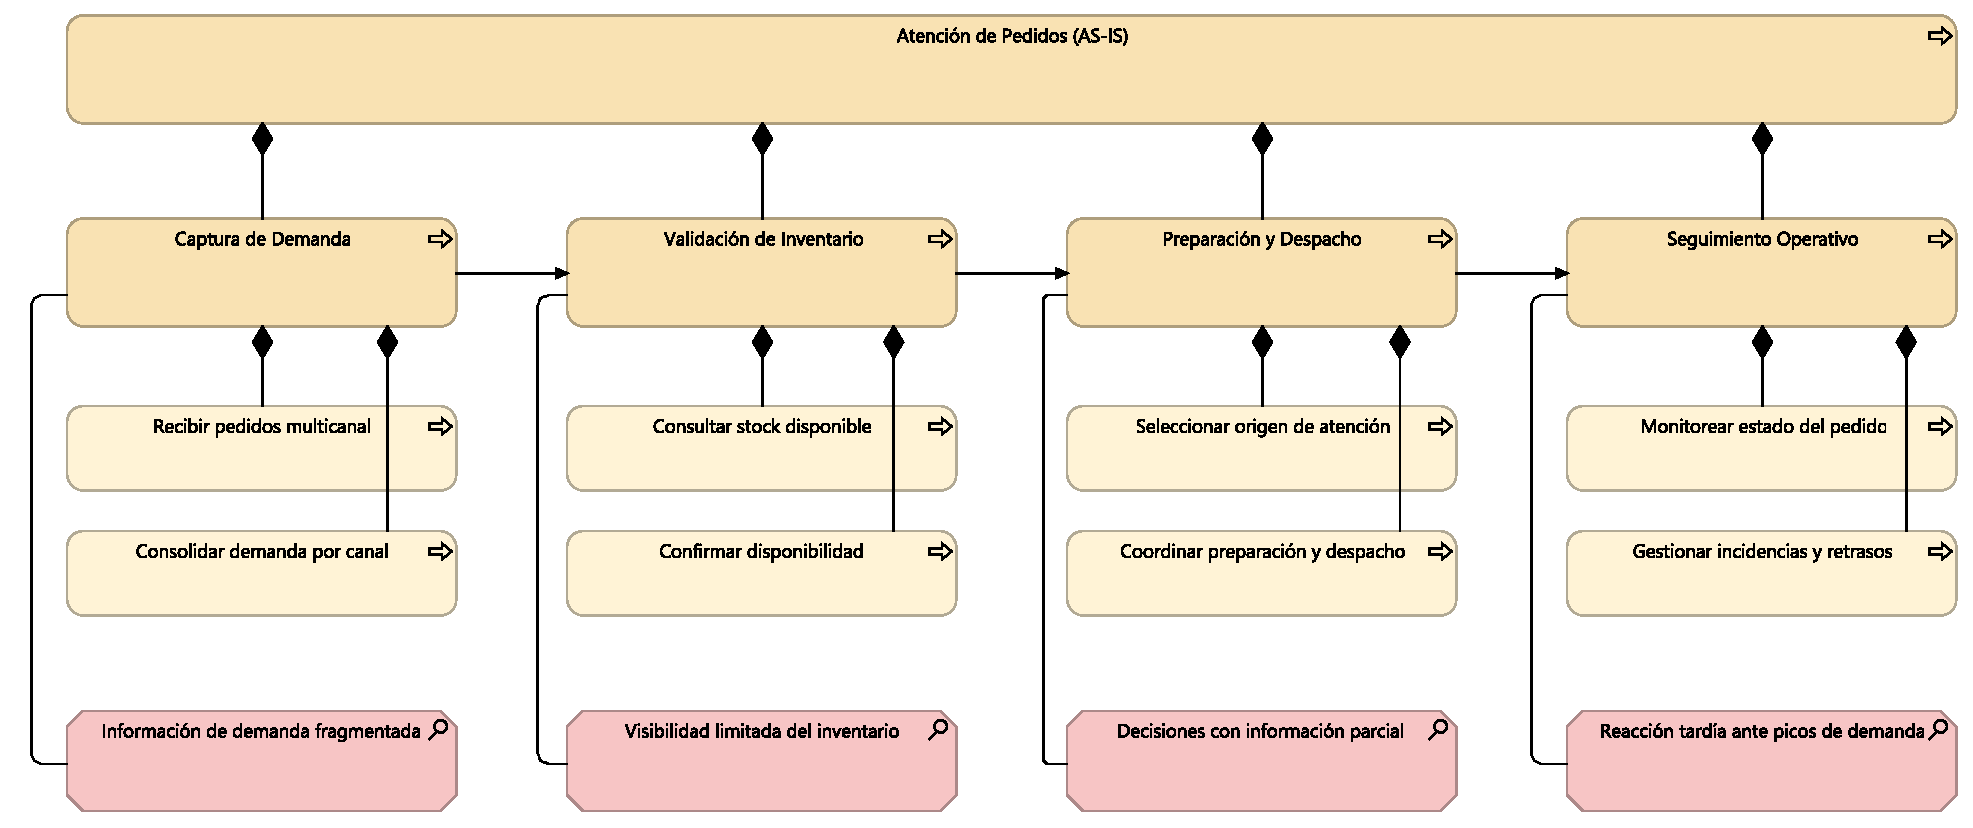
\includegraphics[width=\linewidth]{03_pedidos_asis.pdf}
\caption[Atención de pedidos en la situación actual]{Atención de pedidos en la situación actual.}\label{fig:proceso-asis}
\Fuente{Modelo de solución elaborado por el equipo~\cite{modelo-solucion}}
\end{figure}

\subsection{Fragmentación de inventarios, silos y congestión logística}
La problemática se consolida en cinco frentes. Primero, conocer el stock actual no permite anticipar dónde y cuándo se agotará. Segundo, disponer de inventario global no garantiza que esté cerca de las zonas donde se concentrará la demanda. Tercero, durante campañas como Black Friday la demanda puede superar la capacidad de preparación y distribución antes de que la organización reaccione. Cuarto, las unidades y canales pueden conocer al cliente de forma fragmentada aun cuando exista una identidad maestra. Quinto, la telemetría puede informar que un activo funciona ahora sin anticipar su degradación.

La plataforma debe reducir estas brechas de información mediante histórico, señales recientes, análisis y predicción; no puede corregir por sí sola falta física de stock, insuficiencia transaccional, errores de reserva, carencia de capacidad logística o fallas de ejecución.
\LuminaSilos

\subsection{Relación entre problemas, causas e impactos}
\begin{table}[H]
\caption{Problemas consolidados, aporte de Lumina y responsabilidad operacional}\label{tab:diagnostico}
\scriptsize
\begin{tabularx}{\linewidth}{@{}P{.18\linewidth}P{.24\linewidth}YY@{}}\toprule
Problema & Frase resumen & Aporte de Lumina & Ecosistema operacional\\\midrule
P1. Riesgo de quiebre & Sé cuánto stock tengo, pero no dónde ni cuándo se va a agotar. & Predicción de consumo, riesgo de quiebre, alertas y recomendaciones. & Mantener stock transaccional, reservas, movimientos y reposición.\\
P2. Desalineación geográfica & Sé dónde está mi stock, pero no si está cerca de donde se concentrará la demanda. & Predicción geográfica y recomendaciones de posicionamiento. & Ejecutar transferencias, abastecimiento, asignación logística y despacho.\\
P3. Saturación operativa & Sé que la demanda está creciendo, pero no cuándo va a superar mi capacidad operativa. & Predicción de saturación, presión operacional y cuellos de botella. & Escalar, priorizar y reasignar recursos de operación.\\
P4. Comportamiento fragmentado & Sé quién es el cliente, pero no entiendo su comportamiento completo entre unidades y canales. & Vista analítica transversal, patrones, segmentos y tendencias. & MDM, CRM y sistemas fuente mantienen identidad y operación.\\
P5. Riesgo de falla de activos & Sé que el equipo funciona ahora, pero no cuándo empezará a degradarse o fallar. & Anomalías, riesgo de falla y recomendación de mantenimiento. & Inspeccionar, mantener, reparar y controlar físicamente activos.\\\bottomrule
\end{tabularx}
\end{table}

Estos problemas forman una cadena coherente: anticipar quiebre, verificar proximidad del inventario a la demanda, estimar si la operación absorberá esa demanda, comprender el comportamiento que la origina y asegurar que la infraestructura física pueda sostenerla. El diagnóstico identifica mecanismos de impacto, sin atribuir a Lumina capacidades transaccionales ni mejoras todavía no observadas.


% ================================================================
\AperturaCapitulo{Objetivos, alcance y criterios de éxito}{03_objetivos_alcance.png}{sec:objetivos}
\subsection{Objetivo general y objetivos específicos}
El objetivo general es mejorar la calidad y oportunidad de las decisiones sobre demanda, inventario, capacidad, cliente y activos mediante una plataforma de datos que integre información heterogénea y genere análisis, predicciones, alertas y recomendaciones.

Los objetivos específicos son: anticipar riesgo de quiebre de stock; estimar la demanda por zona para apoyar el posicionamiento de inventario; detectar riesgo de saturación operativa; consolidar una visión analítica del comportamiento del cliente a partir de una identidad confiable; y anticipar degradación de activos. El éxito requiere una secuencia completa desde el dato hasta una decisión registrada, sin trasladar a la plataforma la ejecución transaccional.

\subsection{Verticales y decisiones de negocio}
Las cuatro verticales se mantienen, pero se interpretan como capacidades complementarias. No existe una relación de uno a uno entre problema y vertical: un mismo problema puede requerir señales recientes, históricos, analítica y predicción.

\begin{table}[H]
\caption{Alineamiento entre problemas de negocio y verticales de Lumina}\label{tab:verticales-problemas}
\scriptsize
\resizebox{\textwidth}{!}{%
\begin{tabular}{@{}p{4.4cm}p{4.0cm}p{4.0cm}p{4.0cm}p{4.0cm}@{}}\toprule
Problema & V1. Decisiones en tiempo real & V2. Planes diarios de inventario & V3. Informes operativos & V4. Mantenimiento proactivo\\\midrule
P1. Riesgo de quiebre & Apoya con señales recientes de stock y demanda. & \textbf{Principal}: predicción de quiebre y necesidad estimada. & Mide quiebres, disponibilidad y evolución. & --\\
P2. Stock lejos de demanda & Apoya con señales de demanda y ubicación. & \textbf{Principal}: predicción geográfica y posicionamiento. & Mide costo, distancia y tiempos de entrega. & --\\
P3. Saturación operativa & \textbf{Principal}: detecta presión y cambios rápidos. & Apoya con previsiones de campañas y demanda. & \textbf{Principal}: analiza capacidad, tiempos y costos. & Apoya si una degradación reduce capacidad.\\
P4. Comportamiento fragmentado & Apoya con clics e interacción reciente. & Puede enriquecer forecast de demanda. & \textbf{Principal}: análisis transversal por cliente y canal. & --\\
P5. Degradación de activos & Apoya con telemetría reciente. & -- & Mide desempeño e incidentes históricos. & \textbf{Principal}: anomalías y mantenimiento predictivo.\\\bottomrule
\end{tabular}}
\end{table}

\begin{table}[H]
\caption{Tipo de procesamiento y pregunta de negocio}\label{tab:kpi}
\small
\begin{tabularx}{\linewidth}{@{}P{.18\linewidth}P{.27\linewidth}P{.18\linewidth}Y@{}}\toprule
Tipo & Pregunta que responde & Horizonte & Ejemplo en Lumina\\\midrule
Streaming & ¿Qué está ocurriendo ahora? & Segundos/minutos & Stock cayendo, demanda creciendo, telemetría anómala.\\
Batch & ¿Qué información debe procesarse de forma consolidada? & Horas/días & Históricos de ventas, inventario y preparación de datasets.\\
Analítico / OLAP & ¿Cómo estamos funcionando? & Histórico/consolidado & Costos, tiempos, conversión y utilización.\\
Predictivo & ¿Qué probablemente ocurrirá? & Futuro & Demanda, quiebre, saturación y falla.\\
Prescriptivo & ¿Qué convendría hacer? & Futuro/decisión & Reposición, redistribución, priorización o alternativa recomendada.\\\bottomrule
\end{tabularx}
\end{table}

La capacidad prescriptiva no constituye una quinta vertical; representa una evolución de las capacidades analíticas y predictivas cuando la salida es una recomendación. La ejecución continúa en el ecosistema operacional.

La figura~\ref{fig:apoyo-capacidades} resume las capacidades, resultados e indicadores propuestos.
\GraficoApoyo{a01_capacidades_e_indicadores}{Capacidades de negocio, resultados esperados e indicadores propuestos.}{fig:apoyo-capacidades}

\subsection{Requisitos funcionales y atributos de calidad}
La solución debe integrar eventos e históricos, relacionar entidades, conservar originales, generar señales y exponer resultados analíticos o predictivos. Debe permitir reproceso, controlar accesos, mostrar vigencia y separar claramente información operacional de inteligencia derivada.

Como atributos de calidad se priorizan oportunidad, consistencia, recuperabilidad, escalabilidad y trazabilidad. El sistema operacional confirma disponibilidad, ejecuta reservas, procesa pedidos, pagos, picking y despachos; Lumina no autoriza por sí sola una venta ni se convierte en dependencia obligatoria del camino transaccional.

\subsection{Indicadores y método de medición}
Para los indicadores de oportunidad se medirá el porcentaje de casos que cumple el tiempo objetivo definido. Como meta inicial, al menos el 95\,\% de las alertas deberá estar disponible dentro del umbral establecido para la carga evaluada. La medición se realizará por intervalos de carga y por tipo de evento, sin ocultar errores o datos tardíos. Los totales se conciliarán a igual granularidad y las señales conservarán entidad, momento y causa. El beneficio se estimará comparando períodos o grupos equivalentes y registrando la actuación; la detección técnica no equivale automáticamente a una incidencia evitada.
\LuminaValor

\subsection{Supuestos, restricciones, dependencias y exclusiones}
Se asumen fuentes accesibles, correspondencias válidas de SKU y ubicación, responsables capaces de actuar y sistemas operacionales que mantienen la autoridad sobre pedidos, inventario, reservas, despacho, pagos y mantenimiento. Para cliente se asume una capacidad externa de MDM o resolución de identidad que proporcione un identificador canónico; Lumina consume esa identidad, pero no la gobierna como registro maestro.

Se mantiene la estrategia híbrida con predominio sintético para validación y al menos un dataset público de referencia. Se excluyen del diseño detallado inicial la sustitución del ERP, OMS, WMS, TMS, CRM, MDM, sistemas de mantenimiento, la ejecución de pagos o despachos y un despliegue productivo multirregión. Las metas y retenciones se ajustarán con datos medidos. La propiedad de los datos permanece en RetailSmart.


% ================================================================
\AperturaCapitulo{Estrategia de datos y escenarios de negocio}{04_estrategia_datos.png}{sec:datos}
\subsection{Inventario y clasificación de fuentes}
La operación objetivo integra fuentes propias de aplicaciones de canal, pedidos y ERP; sensores de tienda y almacén; GPS de reparto y telemetría de refrigeración. Cada registro debe conservar fuente, tiempo y entidad. Los datos de interacción explican cambios recientes de demanda; pedidos e inventario sustentan planificación y conciliación; logística y telemetría permiten reconocer desvíos de ejecución o condición.

\subsection{Evaluación de datasets públicos de referencia}
\begin{table}[H]
\caption{Utilidad y límites de los datasets públicos}\label{tab:datasets}
\small\begin{tabularx}{\linewidth}{@{}P{.20\linewidth}YY@{}}\toprule
Dataset & Aplicación de referencia & Límite de interpretación\\\midrule
Olist & Pedidos y contexto logístico; candidato para análisis de entregas y flete & Sus clientes y productos no equivalen a los de otras fuentes.\\
UCI Online Retail & Transacciones por producto y fecha para patrones de compra & No representa GPS, sensores ni condición de activos.\\
theLook eCommerce & Estructura de comercio electrónico disponible en BigQuery & Es público y sintético; no es observación real de RetailSmart.\\\bottomrule
\end{tabularx}
\end{table}
La evaluación identifica dónde aporta cada conjunto; no demuestra representatividad del negocio. El origen sintético de theLook está documentado por Google. UCI describe transacciones de un comercio británico y Olist publica su conjunto en Kaggle~\cite{thelook,uci,olist}.

\subsection{Estrategia híbrida con predominio sintético}
La validación usará escenarios reproducibles para controlar tasas, anomalías y relaciones entre entidades. Un histórico público aportará estructura y una referencia transaccional; Olist es un candidato para el escenario logístico y UCI para ventas. En producción, estos conjuntos se sustituyen por fuentes empresariales. El histórico público y el generador no se presentarán como datos reales de los clientes de RetailSmart.
\LuminaFuentes

\subsection{Correspondencia entre fuentes, entidades y verticales}
Las entidades principales son producto, ubicación, pedido, envío, activo y tiempo. SKU y ubicación relacionan disponibilidad con demanda; pedido o envío relaciona transacciones con tracking; activo y ubicación vinculan telemetría con operación. La matriz del anexo~\ref{anexo:matriz} detalla esta correspondencia. Una fuente puede servir a varias verticales sin duplicar su definición ni atribuirle cobertura que no posee.

\subsection{Escenarios controlados}
\begin{table}[H]
\caption{Escenarios de validación y respuesta esperada}\label{tab:escenarios}
\small\begin{tabularx}{\linewidth}{@{}P{.21\linewidth}YY@{}}\toprule
Escenario & Condición controlada & Comprobación\\\midrule
Operación normal & Stock y condiciones estables & Flujo conciliado y ausencia de alertas injustificadas.\\
Alta demanda & Mayor tasa de clics y descenso de stock correlacionado & Señal oportuna y backlog que se recupera.\\
Anomalía de activo & Temperatura que supera un umbral configurable & Activo, evidencia y responsable de revisión identificados.\\\bottomrule
\end{tabularx}
\end{table}

\subsection{Claves y reglas de correspondencia}
\Vinetta{v02_claves_con_correspondencia.png}{Los datasets se conservan independientes. No se unen clientes o productos por coincidencia de identificador, descripción o importe. El generador puede tomar un catálogo seleccionado y registrar un mapa versionado hacia los SKU del escenario. Un registro sin equivalencia sustentada se mantiene separado y se marca como tal. Antes de cruzar varias observaciones con una venta se agrega a una granularidad compatible para evitar multiplicar importes.}
La figura~\ref{fig:apoyo-correspondencias} sintetiza la independencia de las fuentes y el uso de correspondencias sustentadas.
\GraficoApoyo{a02_correspondencias_validas}{Uso independiente de las fuentes y validación de equivalencias del escenario.}{fig:apoyo-correspondencias}

% ================================================================
\AperturaCapitulo{Arquitectura de Solución de extremo a extremo}{05_arquitectura_solucion.png}{sec:arquitectura}
\subsection{Principios y decisiones de diseño}
El diseño preserva la autoridad de los sistemas operativos, desacopla publicación y consumo, conserva evidencia de origen y separa calidad de datos de su uso. El cómputo continuo se reserva a decisiones cuya utilidad disminuye con la demora. El procesamiento batch consolida históricos y planes. Las responsabilidades lógicas no obligan a crear un servicio o job independiente por cada caja del diagrama.

La Arquitectura de Solución documenta las decisiones arquitectónicas y su correspondencia con componentes, flujos, contratos y tecnologías. Sus vistas representan el modelo de solución. ArchiMate puede utilizarse como notación de modelado. El catálogo y las especificaciones de contratos se mantienen consistentes con el diseño aprobado y con su versión.

\subsection{Vista de negocio y relación con las verticales}
La atención inteligente de pedidos se interpreta como una secuencia de observación, análisis y recomendación sobre una operación que continúa siendo ejecutada por los sistemas transaccionales. V1 aporta conciencia situacional mediante señales recientes; V2 anticipa demanda y necesidades de inventario; V3 explica desempeño y comportamiento transversal; V4 anticipa degradación de activos. Estas capacidades pueden converger sobre un mismo problema sin convertir a Lumina en el ejecutor de la acción.

La figura~\ref{fig:proceso-tobe} vincula estas capacidades con el recorrido del pedido.
\begin{figure}[!htbp]
\centering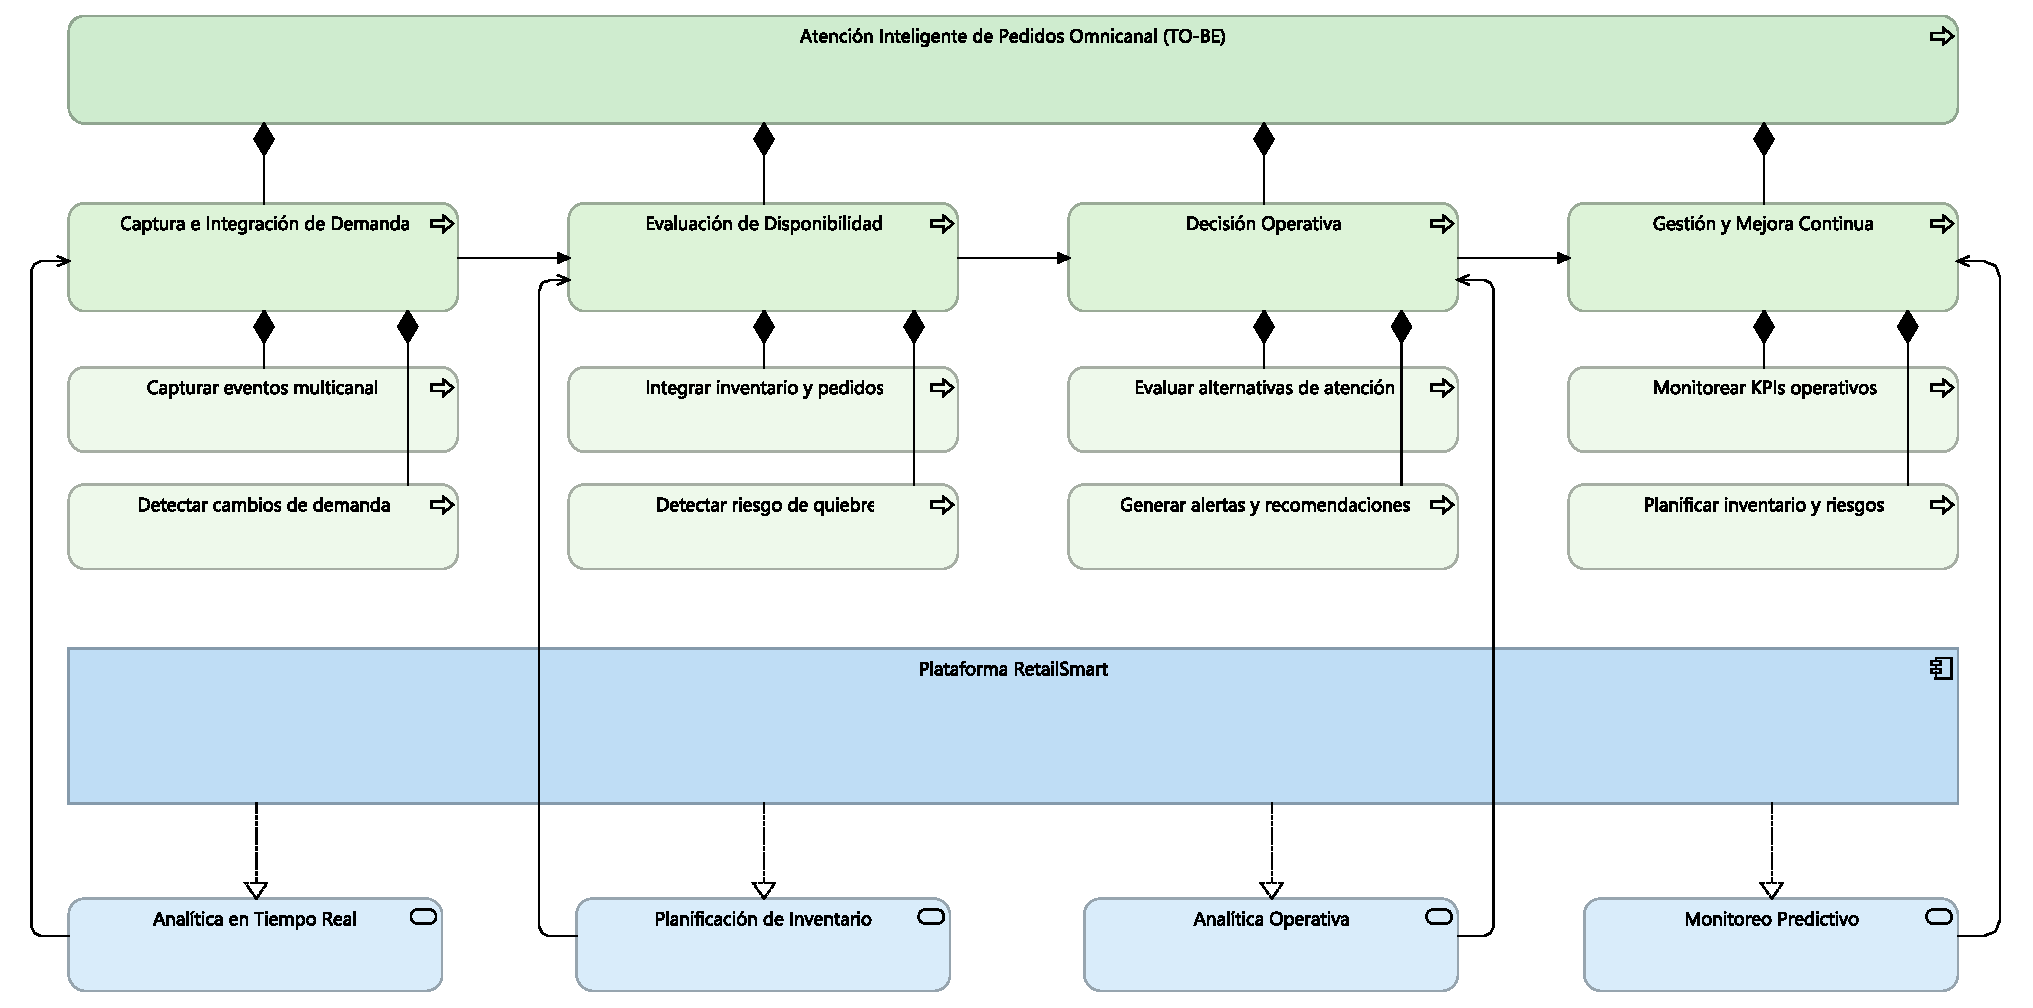
\includegraphics[width=\linewidth]{04_pedidos_tobe.pdf}
\caption[Atención inteligente de pedidos propuesta]{Atención inteligente de pedidos propuesta.}\label{fig:proceso-tobe}
\Fuente{Modelo de solución elaborado por el equipo~\cite{modelo-solucion}}
\end{figure}

\subsection{Vista de aplicaciones y servicios de datos}
Canales, pedidos, ERP, almacenes, logística, CRM, MDM y mantenimiento conservan sus funciones operacionales. La plataforma recibe datos y eventos y entrega señales, planes, indicadores, predicciones y recomendaciones. Los consumidores deben conocer vigencia, calidad y contexto antes de actuar.

Las consultas o APIs posteriores exponen productos de información; una reserva, un pago, una orden de picking, una asignación de vehículo, un cambio de despacho o una intervención de mantenimiento sigue requiriendo validación y ejecución en el sistema transaccional correspondiente. Las vistas completas de aplicaciones frente a procesos se incluyen en el anexo~\ref{anexo:vistas}.

\subsection{Vista tecnológica y correspondencia con GCP}
\begin{table}[H]
\caption{Correspondencia entre componentes de solución y servicios}\label{tab:componentes}
\small\begin{tabularx}{\linewidth}{@{}P{.32\linewidth}YY@{}}\toprule
Componente de solución & Materialización prevista & Responsabilidad\\\midrule
Tópico Eventos Retail & Pub/Sub & Desacoplar productores de consumidores.\\
Procesamiento Streaming & Apache Beam en Dataflow & Validar, normalizar y evaluar reglas o ventanas.\\
Bronze Eventos Raw & Cloud Storage & Conservar payload y origen.\\
Silver Eventos Curados & Cloud Storage y Parquet & Mantener datos integrables y controlados.\\
Tópico Insights Retail & Pub/Sub & Distribuir señales de negocio.\\
Gold Insights Retail & BigQuery & Preparar resultados de consulta y exposición.\\\bottomrule
\end{tabularx}
\end{table}

\subsection{Recorrido por ingesta, procesamiento, almacenamiento y exposición}
La figura~\ref{fig:arquitectura-vector} resume el flujo sin sustituir las vistas detalladas de la Arquitectura de Solución. La persistencia raw y la evaluación de señales pueden avanzar en paralelo, coordinadas por identidad y conciliación. No es necesario leer un archivo Bronze para producir cada alerta. La exposición integra resultados mediante consultas y servicios de datos.
\begin{figure}[!htbp]
\centering
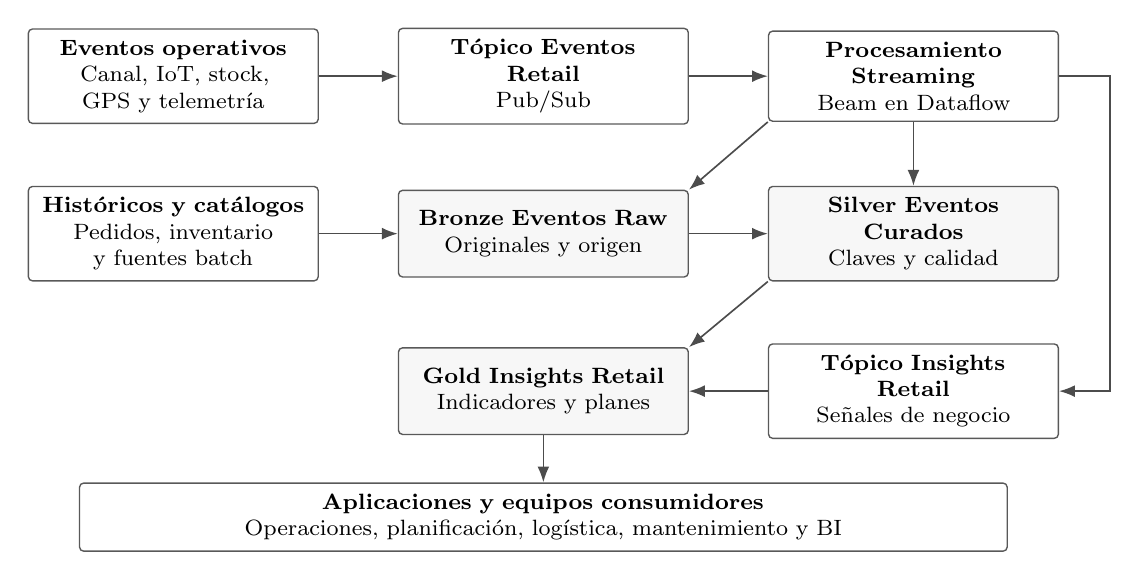
\begin{tikzpicture}[x=1cm,y=1cm,>=Latex,font=\footnotesize,
 caja/.style={draw=black!65,line width=.5pt,rounded corners=1.5pt,align=center,text width=3.4cm,minimum height=1.1cm,inner sep=4pt},
 dato/.style={caja,fill=black!3},linea/.style={->,draw=black!70,line width=.6pt}]
\node[caja] (eventos) at (0,0) {\textbf{Eventos operativos}\\Canal, IoT, stock,\\GPS y telemetría};
\node[caja] (topic) at (4.7,0) {\textbf{Tópico Eventos\\Retail}\\Pub/Sub};
\node[caja] (stream) at (9.4,0) {\textbf{Procesamiento\\Streaming}\\Beam en Dataflow};
\node[caja] (hist) at (0,-2) {\textbf{Históricos y catálogos}\\Pedidos, inventario\\y fuentes batch};
\node[dato] (bronze) at (4.7,-2) {\textbf{Bronze Eventos Raw}\\Originales y origen};
\node[dato] (silver) at (9.4,-2) {\textbf{Silver Eventos\\Curados}\\Claves y calidad};
\node[dato] (gold) at (4.7,-4) {\textbf{Gold Insights Retail}\\Indicadores y planes};
\node[caja] (insights) at (9.4,-4) {\textbf{Tópico Insights\\Retail}\\Señales de negocio};
\node[caja,text width=11.5cm,minimum height=.85cm] (consumo) at (4.7,-5.6) {\textbf{Aplicaciones y equipos consumidores}\\Operaciones, planificación, logística, mantenimiento y BI};
\draw[linea] (eventos)--(topic);
\draw[linea] (topic)--(stream);
\draw[linea] (stream.east) -- ++(.65,0) |- (insights.east);
\draw[linea] (hist)--(bronze);
\draw[linea] (stream.south west)--(bronze.north east);
\draw[linea] (stream)--(silver);
\draw[linea] (bronze)--(silver);
\draw[linea] (silver.south west)--(gold.north east);
\draw[linea] (insights)--(gold);
\draw[linea] (gold)--(consumo);
\end{tikzpicture}
\caption[Síntesis vectorial de la arquitectura de datos]{Síntesis vectorial de la arquitectura de datos. Las flechas expresan flujos lógicos de captura, curación, análisis y exposición.}\label{fig:arquitectura-vector}
\Fuente{síntesis propia alineada con el modelo de solución~\cite{modelo-solucion}}
\end{figure}

\subsection{Trazabilidad entre elementos, componentes y requisitos}
La trazabilidad sigue la secuencia problema, capacidad, componente, dato y validación. Por ejemplo, baja visibilidad de stock se vincula a disponibilidad por SKU y ubicación, a ingesta de \ID{stock\_event}, a curación y a una señal verificable. El catálogo de recursos preserva el identificador lógico y el nombre físico. Las matrices anexas permiten seguir la relación entre fuentes, componentes y resultados.

% ================================================================
\AperturaCapitulo{Diseño detallado de ingesta e integración}{06_ingesta_integracion.png}{sec:ingesta}
\subsection{Criterios para seleccionar batch o streaming}
Streaming se usa cuando la demora cambia la decisión, como riesgo de quiebre o condición de un activo. Batch se usa para consolidación, reconciliación y planes diarios. La selección considera frecuencia del origen, granularidad y tiempo útil del resultado. Se evita exigir baja latencia a una fuente que solo dispone de una actualización diaria.

\subsection{Flujo streaming y contratos de eventos}
Los productores publicarán los seis tipos definidos por la arquitectura en el Tópico Eventos Retail. La validación y normalización producirán datos curados y las reglas generarán señales hacia el Tópico Insights Retail y Gold. Un contrato debe identificar entidad, origen, versión y tiempo. El perfil semántico del anexo es ilustrativo; no modifica los contratos vigentes del repositorio.
\begin{table}[H]
\caption{Eventos de entrada y uso principal}\label{tab:eventos}
\small\begin{tabularx}{\linewidth}{@{}P{.34\linewidth}YY@{}}\toprule
Evento & Fuente & Uso principal\\\midrule
\path{clic_event} & Canal digital & Cambios de interés e interacción.\\
\path{iot_event} & Sensores de tienda & Condiciones de operación.\\
\path{stock_event} & Inventario instrumentado & Disponibilidad por SKU y ubicación.\\
\path{location_event} & GPS & Posición y avance del envío.\\
\path{telemetry_event} & Refrigeración & Condición de activos.\\
\path{warehouse_sensor_event} & Almacén & Condiciones y riesgo operativo.\\\bottomrule
\end{tabularx}
\end{table}

\subsection{Flujo batch y fuentes históricas}
Las cargas de pedidos, inventario y catálogo conservarán un identificador de lote, fuente, fecha y totales. Bronze recibe el archivo o extracción original; la transformación valida y consolida Silver; las agregaciones y estructuras analíticas preparan Gold. La disponibilidad del plan diario se coordinará con la ventana de llegada del origen. Una carga incompleta no se publica como período cerrado.

\subsection{Validación, metadatos y versionamiento de esquemas}
Se comprueban campos obligatorios, tipos, rangos, unidades y claves de referencia. El payload original y el motivo de incumplimiento permiten investigar. La compatibilidad de un nuevo esquema se revisa antes de cambiar productores o consumidores. Se registran tiempo de ocurrencia y tiempo de ingesta para medir oportunidad sin confundir retraso del origen con demora del pipeline.
\Vinetta{v01_tiempo_del_dato.png}{El tiempo de ocurrencia y el de ingesta permiten distinguir vigencia del dato y demora del pipeline.}

\subsection{Duplicados, eventos tardíos, errores y reprocesamiento}
\Vinetta{v03_duplicado_controlado.png}{El identificador estable del evento y las escrituras idempotentes evitan efectos equivalentes repetidos. Se evaluarán ventanas de 30 segundos y una tolerancia inicial de dos minutos; las cifras permanecen configurables. La secuencia de origen o la vigencia impiden que un stock atrasado sustituya un estado más reciente. Dataflow no garantiza una única llamada externa aunque controle resultados dentro del procesamiento~\cite{exactlyonce}. Los inválidos se separan en una ruta controlada, sin añadir tipos de evento.}
La figura~\ref{fig:apoyo-recorrido} resume las responsabilidades lógicas y el tratamiento de excepciones.
\clearpage
\GraficoApoyoDenso{a03_recorrido_y_excepciones}{Recorrido lógico de un evento: preservación, validación, identidad, vigencia y reproceso.}{fig:apoyo-recorrido}

\subsection{Frecuencias, latencias y volúmenes estimados}
Se propone una prueba nominal de \TasaNormal{} eventos/s de \TamEventoKiB{} KiB y un pico de \TasaPico{} eventos/s durante dos horas al día por tres días. La meta inicial es que al menos el 95\,\% de las alertas esté disponible en no más de un minuto bajo carga nominal, y que el plan diario esté disponible antes de las 07:00 de Lima. El intervalo de archivo, el tamaño de lote y la frecuencia de extracción se ajustarán con mediciones; el número de clientes no determina por sí solo la tasa de eventos.

% ================================================================
\AperturaCapitulo{Diseño de almacenamiento y organización de datos}{07_almacenamiento.png}{sec:almacenamiento}
\subsection{Justificación de los motores de almacenamiento}
La propuesta combina un Data Lake de archivos con un Data Warehouse analítico. Cloud Storage conserva originales y Parquet curado; BigQuery organiza consultas y productos de consumo. Esta separación permite reprocesar sin reconstruir el origen y optimizar consultas sin trasladar toda la operación a un motor transaccional. Las capas Medallion por sí solas no constituyen un lakehouse transaccional.

\subsection{Responsabilidad de Bronze, Silver y Gold}
\begin{table}[H]
\caption{Responsabilidades de las capas de datos}\label{tab:medallion}
\small\begin{tabularx}{\linewidth}{@{}P{.14\linewidth}YY@{}}\toprule
Capa & Contenido & Condición de publicación\\\midrule
Bronze & Payloads y archivos originales con origen & Recepción identificada y evidencia recuperable.\\
Silver & Datos normalizados con claves y unidades consistentes & Reglas de calidad y correspondencia conocidas.\\
Gold & Señales, planes e indicadores por granularidad de negocio & Definición del indicador, vigencia y permisos de consumo.\\\bottomrule
\end{tabularx}
\end{table}

\LuminaCapas

\subsection{Formatos, particionamiento y organización física}
Bronze conserva JSON y formatos originales. Silver usa Parquet para lectura selectiva y compresión; se organiza por fuente, tipo y fecha del evento. Gold particiona por fecha del negocio y agrupa por claves utilizadas en consultas. Se propone compactar archivos para evitar objetos pequeños y separar temporales técnicos. Región de cómputo y ubicaciones de datos deben ser compatibles.

\subsection{Retención y ciclo de vida}
Se proponen 30 días en Bronze, 90 días en Silver y 12 meses de resultados Gold para el piloto. Las retenciones deberán validarse según auditoría y recuperación. Bronze será de escritura añadida a nivel lógico; la inmutabilidad exige permisos y política de conservación. La retención no debe impedir el cumplimiento de las políticas de eliminación y privacidad. El archivo histórico de largo plazo se decidirá con una necesidad explícita.

\subsection{Modelo conceptual y estructuras para consumo}
Las entidades son producto, ubicación, pedido, envío, activo y fecha. Los hechos de pedido y entrega se relacionan con dimensiones compartidas; señales y telemetría conservan su propia granularidad. Los productos Gold comprenden disponibilidad y alertas por entidad, plan diario de inventario, indicadores operativos y condición de activos. Cada producto registra fecha de actualización y cobertura de datos.
La figura~\ref{fig:apoyo-entidades} representa las relaciones conceptuales y conserva la granularidad definida.
\GraficoApoyo{a04_entidades_y_granularidad}{Entidades de negocio y relaciones conceptuales descritas en el diseño aprobado.}{fig:apoyo-entidades}

\subsection{Integración del histórico con eventos operativos}
Los eventos enriquecen la visión reciente y el histórico permite contexto y conciliación. La unión se realiza sobre claves válidas y una referencia temporal compatible. Antes de cruzar varios eventos con una transacción se agrega al nivel de la venta. La conversión exige una relación sustentada entre interacción y compra; en ausencia de esa relación se muestran ambas métricas por separado.

% ================================================================
\AperturaCapitulo{Selección y justificación tecnológica}{08_seleccion_tecnologica.png}{sec:tecnologia}
\subsection{Criterios y alternativas consideradas}
La comparación considera oportunidad de la decisión, esfuerzo de operación, portabilidad, seguridad y mantenibilidad. Se evalúa una base gestionada en GCP frente a una plataforma autogestionada con componentes abiertos. La primera reduce tareas de operación, mientras la segunda ofrece mayor control a cambio de desplegar, actualizar, dimensionar y recuperar más infraestructura. Ninguna alternativa elimina la necesidad de gobierno o soporte.
\begin{table}[H]
\caption{Alternativas tecnológicas y compromisos}\label{tab:alternativas}
\small\begin{tabularx}{\linewidth}{@{}P{.21\linewidth}YY@{}}\toprule
Decisión & Opción del diseño & Alternativa y compromiso\\\midrule
Mensajería & Pub/Sub; desacoplamiento sin administrar brokers & Kafka; mayor control y portabilidad del protocolo, con operación propia o capacidad gestionada.\\
Streaming & Apache Beam en Dataflow & Otro runner o Flink; revisar conectores, estado y semántica de recuperación.\\
Archivos & Cloud Storage con formatos abiertos & Almacenamiento compatible con objetos; revisar garantías y operación.\\
Analítica & BigQuery para Gold y consultas SQL & Motor abierto como Trino; requiere organizar capacidad y operación.\\\bottomrule
\end{tabularx}
\end{table}

\subsection{Sustento de los componentes seleccionados}
Pub/Sub permite desacoplar productores y consumidores; Beam expresa transformaciones y ventanas; Dataflow ejecuta el procesamiento gestionado; Cloud Storage conserva archivos y BigQuery organiza consultas. La decisión distribuye responsabilidades por capa y evita usar un almacén analítico para coordinar transacciones. El motor batch definitivo se ajustará al volumen; no se despliega un clúster permanente sin una carga que lo justifique~\cite{pubsub,beam}.

\subsection{Tecnologías abiertas y servicios administrados de GCP}
RetailSmart ha expresado una preferencia por tecnologías abiertas. Python, Beam, Parquet y lógica SQL portable atienden parte de ese objetivo. Pub/Sub, Dataflow, Cloud Storage y BigQuery son servicios propietarios; usar clientes abiertos no los convierte en software abierto. Por ello, la arquitectura gestionada requiere una decisión explícita sobre la dependencia de plataforma. Si la prioridad es evitar dependencia de proveedor, se deberá comparar una alternativa abierta antes de consolidar la implementación.

\subsection{Compromisos de portabilidad, rendimiento y operación}
Se acepta dependencia de servicio a cambio de reducir operación inicial. La salida se facilita con formatos abiertos, metadatos exportables, lógica separada de conectores y contratos versionados, sin prometer migración automática. Se revisará el enfoque si las restricciones de residencia o la política de software superan el beneficio de la gestión delegada. Los modelos predictivos se incorporan solo si superan un baseline simple y justifican su mantenimiento.

\subsection{Registro de decisiones de arquitectura}
\begin{table}[H]
\caption{Decisiones y condiciones de aceptación}\label{tab:adr}
\small\begin{tabularx}{\linewidth}{@{}P{.12\linewidth}YY@{}}\toprule
ID & Decisión de diseño & Consecuencia o condición\\\midrule
ADR 01 & Integración híbrida y escenarios sintéticos controlados & Se complementa con un histórico público; el impacto real exige piloto operativo.\\
ADR 02 & Bronze y Silver en objetos; Gold analítico & Separar evidencia de preparación y consumo.\\
ADR 03 & Identidad estable e idempotencia & Reproceso sin duplicar efectos de negocio.\\
ADR 04 & Despliegue regional inicial & La recuperación ante pérdida de región requiere una copia externa y un procedimiento probado.\\
ADR 05 & Uso de servicios GCP gestionados & Excepción pendiente frente al mandato de código abierto.\\\bottomrule
\end{tabularx}
\end{table}
La figura~\ref{fig:apoyo-decision} muestra la secuencia para actualizar el diseño y su documentación antes de modificar la implementación.
\GraficoApoyo{a05_decision_y_actualizacion}{Secuencia de actualización del diseño antes de modificar la implementación.}{fig:apoyo-decision}

% ================================================================
\AperturaCapitulo{Escalabilidad y rendimiento}{09_escalabilidad.png}{sec:escala}
\subsection{Volumetría y carga normal}
El escenario de referencia utiliza 20 eventos/s de \TamEventoKiB{} KiB durante 30 días. Esto equivale a 51,84 millones de eventos y aproximadamente 74,2 GiB de payload raw mensual. Son parámetros de un piloto acotado, no una extrapolación desde nueve millones de clientes. El número de workers es una hipótesis de capacidad que debe validarse.

\subsection{Black Friday y Cyber Monday}
Se propone aumentar a 400 eventos/s durante dos horas al día por tres días, manteniendo igual tamaño medio. El mes resultante contiene aproximadamente 60,05 millones de eventos. La prueba observa aumento de demanda, descenso correlacionado de stock y acumulación logística. Además de la latencia durante el pico, se mide cuánto tarda en vaciarse el trabajo pendiente una vez que la tasa retorna a normalidad.

\subsection{Capacidad y escalamiento por capa}
\begin{table}[H]
\caption{Controles de capacidad por capa}\label{tab:capacidad}
\small\begin{tabularx}{\linewidth}{@{}P{.20\linewidth}YY@{}}\toprule
Capa & Señal a observar & Acción a evaluar\\\midrule
Productores y captura & Errores de publicación, cuota y reintentos & Regular tasa y tamaño de lote; evitar pérdida silenciosa.\\
Streaming & Backlog, tiempo de respuesta de alertas, CPU y claves calientes & Revisar paralelismo, ventanas y límites de workers.\\
Archivos & Archivos pequeños y demora de escritura & Ajustar tamaño y frecuencia de consolidación.\\
Gold y consultas & Demora y bytes escaneados & Particionar, seleccionar columnas y preparar agregados.\\\bottomrule
\end{tabularx}
\end{table}

\subsection{Cuellos de botella y saturación}
\Vinetta{v04_evento_tardio.png}{Un backlog creciente puede originarse en claves concentradas, un destino lento, cuotas o lógica de procesamiento intensiva. Añadir workers no resuelve necesariamente el límite del destino. Se revisará el tramo que acumula trabajo antes de incrementar capacidad. La retención protege una ventana de recuperación, pero no representa almacenamiento ilimitado. Batch y consultas masivas se programarán para no competir innecesariamente con decisiones urgentes.}

\subsection{Objetivos y pruebas de rendimiento}
La meta nominal es que al menos el 95\,\% de las alertas esté disponible en $\leq60$ s, acompañada de conciliación y registro de errores. Para el pico se verificará crecimiento y recuperación del backlog sin pérdida no explicada; el umbral de latencia de campaña se acordará con la necesidad operativa. El escenario de prueba contempla dos workers de 2 vCPU y 8 GiB y hasta ocho durante seis horas de pico. Esta capacidad debe confirmarse experimentalmente.
La figura~\ref{fig:apoyo-carga} sintetiza los escenarios de carga propuestos y sus condiciones de validación.
\GraficoApoyo{a06_escenarios_de_carga}{Escenarios nominal y pico propuestos para validar el comportamiento del flujo.}{fig:apoyo-carga}

% ================================================================
\AperturaCapitulo{Justificación económica y estimación de costos}{15_analisis_costos.png}{sec:costos}

La arquitectura TO-BE de Lumina Retail se evalúa económicamente a partir de los componentes que soportan la ingesta, el procesamiento, el almacenamiento y el consumo analítico. La estimación diferencia los precios públicos de Google Cloud de los supuestos de dimensionamiento utilizados para el escenario inicial.

\begin{quote}
\small
\textbf{Nota de estimación.} Los precios unitarios corresponden a tarifas públicas de Google Cloud consultadas a octubre de 2026. Los volúmenes, workers y patrones de consulta son supuestos de dimensionamiento del proyecto y no representan datos productivos reales de RetailSmart. Los montos son estimaciones referenciales y pueden variar por configuración, operaciones auxiliares, transferencia de datos, servicios complementarios, descuentos por compromiso y acuerdos comerciales. Dado el tamaño de RetailSmart y su crecimiento exponencial, un convenio empresarial o compromiso de consumo con Google Cloud podría reducir los precios efectivos frente a las tarifas públicas utilizadas.
\end{quote}

\subsection{Estructura de costos de la arquitectura}
Los costos se organizan según la capacidad técnica que soportan dentro de la solución.

\begin{table}[H]
\caption{Estructura de costos de Lumina Retail}\label{tab:estructura-costos}
\small
\begin{tabularx}{\linewidth}{@{}P{.27\linewidth}P{.36\linewidth}Y@{}}\toprule
Grupo & Propósito & Componentes principales\\\midrule
A. Ingesta y mensajería & Recibir y desacoplar eventos operacionales & Pub/Sub\\
B. Procesamiento streaming & Procesar eventos de baja latencia & Dataflow / Apache Beam\\
C. Almacenamiento Data Lake & Conservar Bronze y Silver & Cloud Storage + Parquet\\
D. Analítica y consumo Gold & Consultas, indicadores y productos analíticos & BigQuery\\
E. Operación y observabilidad & Logs, métricas, monitoreo y soporte & Cloud Logging, Monitoring, discos y servicios auxiliares\\
F. Procesamiento batch & Cargas históricas, planes diarios y reprocesos & Jobs batch bajo demanda\\
G. Crecimiento y campañas & Absorber expansión del negocio y picos & Autoscaling, mayor volumen y consultas\\\bottomrule
\end{tabularx}
\end{table}

\subsection{Supuestos de dimensionamiento}
La estimación base corresponde a un escenario inicial de validación de la arquitectura. Estos valores deberán recalibrarse con telemetría real antes de producción.

\begin{table}[H]
\caption{Supuestos utilizados para la estimación económica}\label{tab:supuestos-costos}
\small
\begin{tabularx}{\linewidth}{@{}P{.48\linewidth}Y@{}}\toprule
Variable & Supuesto\\\midrule
Carga nominal & 20 eventos/s\\
Eventos mensuales nominales & 51.84 millones\\
Payload raw mensual & 74.2 GiB\\
Pico de campaña & 400 eventos/s\\
Duración del pico & 2 h/día durante 3 días\\
Dataflow nominal & 2 workers streaming\\
Dataflow pico & hasta 8 workers\\
Worker de referencia & 4 vCPU + 15 GiB RAM\\
Silver & 50\% de Bronze\\
Gold & 20\% de Bronze\\
Consultas BigQuery & 2 TiB/mes\\\bottomrule
\end{tabularx}
\end{table}

\subsection{Precios unitarios de referencia}
Las tarifas utilizadas corresponden a precios públicos de referencia y sirven como base para los cálculos del escenario.

\begin{table}[H]
\caption{Precios unitarios utilizados}\label{tab:precios-gcp-costos}
\small
\begin{tabularx}{\linewidth}{@{}P{.25\linewidth}P{.40\linewidth}Y@{}}\toprule
Servicio & Unidad & Tarifa utilizada\\\midrule
Pub/Sub & Throughput después de 10 GiB/mes gratuitos & USD 40/TiB\\
Dataflow streaming & vCPU & USD 0.069/h\\
Dataflow streaming & Memoria & USD 0.003557/GiB-h\\
Dataflow Streaming Engine & Unidad de cómputo & USD 0.089/unidad\\
Cloud Storage Standard & Almacenamiento regional & aprox. USD 0.020/GiB-mes\\
BigQuery on-demand & Después de 1 TiB/mes gratuito & USD 6.25/TiB\\
BigQuery active logical storage & Después de 10 GiB/mes gratuitos & aprox. USD 0.023/GiB-mes\\\bottomrule
\end{tabularx}
\end{table}

\subsection{Ingesta y mensajería}
Para Pub/Sub se considera una publicación y una entrega principal al consumidor streaming. El volumen mensual estimado es 148.4 GiB entre publicación y entrega.

\[
\frac{148.4-10}{1024}\times 40 \approx \text{USD }5.41/\text{mes}
\]

\begin{table}[H]
\caption{Costo estimado de ingesta y mensajería}\label{tab:costo-pubsub}
\small
\begin{tabularx}{\linewidth}{@{}XY@{}}\toprule
Concepto & Estimado mensual\\\midrule
Pub/Sub & USD 5.41\\\bottomrule
\end{tabularx}
\end{table}

El costo de mensajería es reducido frente al cómputo y aumenta principalmente con el volumen procesado.

\subsection{Procesamiento streaming}
El procesamiento de baja latencia representa el principal componente cuantificable del escenario base.

\[
2\times730\times[(4\times0.069)+(15\times0.003557)]
\approx \text{USD }480.86/\text{mes}
\]

Para el pico se consideran seis workers adicionales durante seis horas acumuladas:

\[
6\times6\times[(4\times0.069)+(15\times0.003557)]
\approx \text{USD }11.86
\]

\begin{table}[H]
\caption{Costo estimado de procesamiento streaming}\label{tab:costo-dataflow}
\small
\begin{tabularx}{\linewidth}{@{}XY@{}}\toprule
Concepto & Estimado mensual\\\midrule
Dataflow nominal: CPU + RAM & USD 480.86\\
Capacidad adicional de pico & USD 11.86\\
\textbf{Subtotal procesamiento streaming} & \textbf{USD 492.72}\\\bottomrule
\end{tabularx}
\end{table}

No se incluyen en este subtotal Streaming Engine, Persistent Disk ni otros consumos que dependen de la ejecución real.

\subsection{Almacenamiento Data Lake}
Bronze conserva aproximadamente 74.2 GiB mensuales. Para Silver se asume una reducción a 50\% del volumen Bronze como efecto de curación y compresión.

\begin{table}[H]
\caption{Costo estimado del Data Lake}\label{tab:costo-datalake}
\small
\begin{tabularx}{\linewidth}{@{}P{.35\linewidth}P{.30\linewidth}Y@{}}\toprule
Capa & Volumen estimado & Costo mensual\\\midrule
Bronze & 74.2 GiB & USD 1.48\\
Silver & 37.1 GiB & USD 0.74\\
\textbf{Subtotal Data Lake} & 111.3 GiB & \textbf{USD 2.22}\\\bottomrule
\end{tabularx}
\end{table}

El almacenamiento representa una proporción menor del escenario base. El uso de Parquet en Silver reduce volumen y lectura.

\subsection{Analítica y consumo Gold}
Para Gold se utiliza como referencia 20\% del volumen Bronze. El escenario de consultas considera 2 TiB/mes, de los cuales 1 TiB se toma como volumen facturable después de la franquicia utilizada en el cálculo.

\begin{table}[H]
\caption{Costo estimado de la capa Gold}\label{tab:costo-gold}
\small
\begin{tabularx}{\linewidth}{@{}XY@{}}\toprule
Concepto & Estimado mensual\\\midrule
Gold storage & USD 0.11\\
Consultas BigQuery & USD 6.25\\
\textbf{Subtotal Gold / Analítica} & \textbf{USD 6.36}\\\bottomrule
\end{tabularx}
\end{table}

El costo analítico depende principalmente de los bytes consultados. El particionamiento, la selección de columnas y los agregados son los principales controles de optimización.

\subsection{Operación y observabilidad}
Los consumos asociados a operación se incorporarán al TCO cuando exista medición del comportamiento real.

\begin{table}[H]
\caption{Costos variables pendientes de medición}\label{tab:costos-observabilidad}
\small
\begin{tabularx}{\linewidth}{@{}P{.38\linewidth}Y@{}}\toprule
Componente & Consideración\\\midrule
Streaming Engine & Precio oficial conocido; consumo pendiente de medición\\
Persistent Disk & Dependiente del job final\\
Cloud Logging & Dependiente del volumen de logs\\
Cloud Monitoring & Dependiente de métricas y retención\\
Transferencia de red & Dependiente de flujo entre regiones y servicios\\
Operaciones Cloud Storage & Dependiente de la cantidad de requests\\\bottomrule
\end{tabularx}
\end{table}

\subsection{Procesamiento batch}
La arquitectura no contempla inicialmente un clúster batch permanente. Las cargas históricas, planes diarios de inventario, conciliaciones, reprocesos y preparación de datasets se ejecutarán bajo demanda.

\begin{quote}
\textbf{Criterio económico:} no mantener capacidad batch permanente mientras la carga no demuestre que es necesaria.
\end{quote}

El costo de esta capacidad se contabilizará según ejecución real y no forma parte del subtotal base.

\subsection{Consolidado mensual}
El escenario cuantificable actual se resume a continuación.

\begin{table}[H]
\caption{Consolidado mensual de costos cuantificables}\label{tab:consolidado-costos}
\small
\begin{tabularx}{\linewidth}{@{}XY@{}}\toprule
Grupo & Estimado mensual\\\midrule
A. Ingesta y mensajería & USD 5.41\\
B. Procesamiento streaming & USD 492.72\\
C. Data Lake & USD 2.22\\
D. Gold / Analítica & USD 6.36\\
E. Operación y observabilidad & Pendiente de medición\\
F. Batch & Variable por ejecución\\\midrule
\textbf{Subtotal cuantificable mensual} & \textbf{USD 506.71}\\\bottomrule
\end{tabularx}
\end{table}

La referencia anual del subtotal cuantificable es:

\[
506.71\times12 \approx \text{USD }6{,}080.50/\text{año}
\]

Este valor no representa el TCO definitivo de la plataforma.

\subsection{Sensibilidad al crecimiento}
RetailSmart opera a gran escala y presenta crecimiento exponencial. La siguiente sensibilidad muestra el efecto del aumento de volumen sobre eventos y almacenamiento; no constituye una predicción comercial.

\begin{table}[H]
\caption{Sensibilidad del volumen ante crecimiento}\label{tab:sensibilidad-costos}
\small
\begin{tabularx}{\linewidth}{@{}P{.28\linewidth}P{.18\linewidth}P{.25\linewidth}Y@{}}\toprule
Escenario & Eventos/s & Eventos/mes & Bronze raw/mes\\\midrule
Base & 20 & 51.84 M & 74.2 GiB\\
5x & 100 & 259.2 M & 371 GiB\\
10x & 200 & 518.4 M & 742 GiB\\
Pico de campaña & 400 & Variable & Variable\\\bottomrule
\end{tabularx}
\end{table}

Pub/Sub y Storage crecen principalmente con el volumen. Dataflow depende de autoscaling, ventanas, estado y lógica del pipeline; BigQuery depende de los bytes efectivamente consultados. Las pruebas de carga deberán preceder cualquier aumento permanente de capacidad.

\subsection{Acuerdos comerciales y compromisos}
La estimación utiliza precios públicos. Para una organización del tamaño de RetailSmart pueden existir compromisos de consumo, contratos empresariales, descuentos por volumen, créditos o condiciones negociadas con Google Cloud.

\begin{table}[H]
\caption{Referencia de compromisos sobre CPU y memoria nominales}\label{tab:descuentos-costos}
\small
\begin{tabularx}{\linewidth}{@{}P{.35\linewidth}P{.25\linewidth}Y@{}}\toprule
Modalidad & Descuento de referencia & CPU + RAM nominal estimado\\\midrule
Sin compromiso & 0\% & USD 480.86/mes\\
Compromiso 1 año & aprox. 20\% & USD 384.69/mes\\
Compromiso 3 años & aprox. 40\% & USD 288.51/mes\\\bottomrule
\end{tabularx}
\end{table}

Estos valores son ilustrativos y no sustituyen una cotización empresarial.

\subsection{Indicadores de eficiencia}
La eficiencia tecnológica puede compararse mediante el costo por millón de eventos:

\[
\text{Costo por millón de eventos}
=
\frac{506.71}{51.84}
\approx \text{USD }9.77
\]

Este indicador no implica que Lumina procese transaccionalmente un pedido. Para negocio, el indicador de referencia es:

\[
\text{Costo operativo por pedido}
=
\frac{\text{preparación + almacenamiento + distribución + última milla}}
{\text{pedidos entregados}}
\]

Lumina busca reducir este indicador mediante menor distancia de última milla, menos reposiciones urgentes, mejor posicionamiento de inventario, anticipación de saturación y mantenimiento proactivo.

\subsection{Controles FinOps}
El control económico de la plataforma se realizará mediante indicadores que permitan relacionar gasto tecnológico y evolución del negocio.

\begin{table}[H]
\caption{Indicadores FinOps propuestos}\label{tab:finops-costos}
\small
\begin{tabularx}{\linewidth}{@{}P{.43\linewidth}Y@{}}\toprule
Indicador & Uso\\\midrule
Costo mensual total & Control presupuestario\\
Costo por vertical & Identificar capacidades costosas\\
Costo por millón de eventos & Medir eficiencia de procesamiento\\
GiB almacenados por capa & Controlar crecimiento Bronze/Silver/Gold\\
TiB consultados en BigQuery & Controlar costo analítico\\
Costo por campaña & Medir impacto de picos\\
Workers promedio y máximo & Evaluar autoscaling\\
Costo operativo por pedido & Relacionar plataforma con valor de negocio\\\bottomrule
\end{tabularx}
\end{table}

\subsection{Conclusión económica}
La estimación muestra que el procesamiento streaming concentra el principal costo cuantificable, mientras que mensajería, almacenamiento y analítica representan una proporción menor. Para una organización grande y en crecimiento, la arquitectura debe mantenerse elástica, observable y económicamente controlable, evitando sobredimensionar permanentemente la capacidad.

La estrategia económica consiste en almacenar eficientemente, utilizar streaming cuando la baja latencia genera valor, ejecutar batch bajo demanda, ampliar capacidad temporalmente en campañas y medir de forma continua el costo unitario.

\subsection{Resumen ejecutivo de costo del proyecto}
A partir de los componentes cuantificables, el escenario base presenta el siguiente presupuesto de referencia:

\begin{table}[H]
\caption{Resumen ejecutivo del costo de infraestructura}\label{tab:resumen-costos}
\small
\begin{tabularx}{\linewidth}{@{}XY@{}}\toprule
Concepto & Estimación\\\midrule
Costo mensual cuantificable & USD 506.71/mes\\
Costo anual cuantificable & USD 6,080.52/año\\
Reserva de planeamiento propuesta (20\%) & USD 1,216.10/año\\
\textbf{Presupuesto anual de referencia para infraestructura} & \textbf{aprox. USD 7,296.62/año}\\\bottomrule
\end{tabularx}
\end{table}

La reserva del 20\% constituye una holgura presupuestaria para consumos aún no medidos —Streaming Engine, discos, logging, operaciones de almacenamiento, batch y servicios auxiliares— y no corresponde a una tarifa de Google Cloud.

\begin{quote}
\textbf{Presupuesto inicial recomendado de infraestructura cloud: USD 600--610 mensuales, equivalente a aproximadamente USD 7.3 mil anuales para el escenario base.}
\end{quote}

Este monto corresponde al costo operativo tecnológico estimado de la plataforma. No incluye horas de implementación, arquitectura, ingeniería de datos, QA, soporte operativo, licencias externas, capacitación, migración de datos ni servicios profesionales.

Por tanto, el TCO completo deberá considerar:

\[
\text{TCO}
=
\text{Infraestructura Cloud}
+
\text{Implementación}
+
\text{Operación y soporte}
+
\text{Licencias}
+
\text{Evolución y mantenimiento}
\]

Para el escenario inicial, RetailSmart debería considerar un presupuesto cloud del orden de \textbf{USD 7,000--7,500 por año}, sujeto a recalibración con datos productivos y a posibles descuentos corporativos con Google Cloud.


\AperturaCapitulo{Fiabilidad, alta disponibilidad y recuperación}{10_fiabilidad_recuperacion.png}{sec:resiliencia}
\subsection{Escenarios de falla y consecuencias operativas}
La solución debe reconocer fuentes caídas, fallas de procesamiento, datos inválidos y pérdida regional. El riesgo principal es que una información incompleta o vencida se consuma como disponibilidad vigente. La respuesta combina marcar degradación, conservar evidencia, controlar salidas y recuperar procesamiento. Alta disponibilidad local y recuperación ante desastre regional son responsabilidades relacionadas, pero distintas.

Como criterio de alta disponibilidad, se evita introducir coordinadores autogestionados de instancia única. Se debe comprobar la cobertura zonal de los servicios elegidos y ensayar el reinicio de workers sin pérdida no explicada. La continuidad ante pérdida completa de región requiere un diseño adicional de recuperación.

\subsection{Indisponibilidad del inventario de una tienda}
Se mantiene la última lectura como referencia y se marca su vigencia. Operaciones debe saber que la fuente está degradada antes de confirmar un compromiso. La venta se valida en el sistema transaccional o mediante una alternativa operativa autorizada. Un heartbeat o una regla de frescura permite proponer detección de indisponibilidad en cinco minutos o menos, pendiente de prueba.
\LuminaContinuidad
La figura~\ref{fig:apoyo-vigencia} presenta una maqueta conceptual para comunicar la vigencia de la fuente sin representar una aplicación implementada.
\GraficoApoyo{a08_maqueta_vigencia_inventario}{Maqueta conceptual para comunicar vigencia y degradación; no representa una aplicación implementada.}{fig:apoyo-vigencia}

\subsection{Tolerancia a fallos y recuperación del procesamiento}
Los mensajes retenidos, los originales y los puntos persistidos permiten retomar el flujo. Se recupera configuración y permisos y se reprocesa con la misma identidad lógica. La conciliación debe comparar entradas, duplicados, rechazados y resultados. Los consumidores de señales también deben controlar repetición; la garantía interna del runner no basta para una acción externa exactamente una vez~\cite{exactlyonce}.

\subsection{Objetivos RTO y RPO propuestos}
\begin{table}[H]
\caption{Objetivos iniciales de recuperación}\label{tab:rto}
\small\begin{tabularx}{\linewidth}{@{}P{.27\linewidth}YY@{}}\toprule
Incidente & Objetivo propuesto & Condición y evidencia\\\midrule
Fuente de inventario caída & Detección $\leq5$ min & Regla de frescura y visibilidad de estado degradado.\\
Job o worker indisponible & RTO $\leq30$ min & Recuperar desde datos ya persistidos y retenidos.\\
Pérdida de región & RTO 4 h y RPO 24 h & Solo tras habilitar y probar una copia fuera de la región.\\\bottomrule
\end{tabularx}
\end{table}
RTO es el tiempo objetivo de recuperación y RPO la pérdida máxima tolerada. Los valores son decisiones propuestas; no son SLA de GCP ni resultados medidos. El despliegue regional inicial no demuestra por sí solo continuidad multirregión.
La figura~\ref{fig:apoyo-recuperacion} sintetiza los objetivos propuestos y las condiciones necesarias para validarlos.
\GraficoApoyo{a07_rto_rpo_y_condiciones}{Objetivos RTO y RPO, condicionados a una copia externa habilitada y probada.}{fig:apoyo-recuperacion}

\subsection{DRP y procedimiento de validación}
El procedimiento identifica el incidente, contiene resultados incorrectos, restaura configuración y acceso, recupera datos y concilia antes de reabrir consumo. El simulacro registra tiempos y diferencias y permite ajustar objetivos. La copia externa a la región deberá habilitarse y probarse según la criticidad del servicio.

% ================================================================
\AperturaCapitulo{Gobierno, calidad y seguridad de datos}{11_gobierno_calidad_seguridad.png}{sec:gobierno}
\subsection{Responsables y clasificación}
RetailSmart conserva la propiedad del dato. Cada dominio debe designar un responsable de definición y calidad y cada producto de información un responsable de consumo. Se propone clasificar los conjuntos según sensibilidad y necesidad operativa, minimizando datos personales. El contrato con el proveedor debe proteger acceso, exportación y continuidad, y dejar clara la titularidad de los datos y de la tecnología.

\subsection{Catálogo, diccionario y metadatos}
El catálogo documenta propósito, fuente, owner o responsable, granularidad, esquema, versión, calidad y consumidores. El diccionario define el significado de campos, unidades y claves. Los metadatos de recepción no sustituyen el tiempo del negocio. En esta fase se propone un catálogo versionado y metadatos obligatorios; la implantación completa de una herramienta gestionada de catálogo se incorpora cuando el alcance lo justifique.

\subsection{Linaje desde la fuente hasta el consumo}
Un indicador o una señal debe poder rastrearse hasta su evento o lote, la transformación aplicada y la versión de regla o modelo. Se conserva la correspondencia entre fuente y entidad del escenario. El linaje lógico se diseña desde el inicio y la evidencia automática se incorpora con los pipelines. Una flecha en el diagrama expresa una relación prevista, no prueba que el linaje técnico ya esté implementado.
\LuminaGobierno

\subsection{Reglas de calidad e incumplimientos}
\Vinetta{v05_calidad_y_origen.png}{Las reglas cubren completitud, tipo, rango, unidad, unicidad, frescura y referencia válida. Se concilian entradas con válidos, duplicados y rechazados usando categorías excluyentes definidas para cada conteo. Un incumplimiento conserva causa y origen y puede impedir publicar un período o activar una señal. Los umbrales se acuerdan con el uso del dato y se revisan con los usuarios.}

\subsection{Identidades, permisos y mínimo privilegio}
\begin{table}[H]
\caption{Separación funcional de accesos}\label{tab:iam}
\small\begin{tabularx}{\linewidth}{@{}P{.24\linewidth}YY@{}}\toprule
Identidad & Acceso necesario & Límite\\\midrule
Aprovisionamiento & Crear y configurar recursos catalogados & No utilizarla como identidad de los jobs.\\
Ejecución Dataflow & Leer entradas y escribir en destinos de su función & Evitar permisos globales de Editor o administración total.\\
Consumo & Consultar productos autorizados & No otorgar acceso general a Bronze o información sensible.\\\bottomrule
\end{tabularx}
\end{table}
Los permisos concretos se asignan al recurso y a la operación necesaria y se verifican mediante pruebas positivas y negativas. La propagación y los agentes gestionados se revisarán durante el bootstrap sin confundirlos con las cuentas de ejecución.

\subsection{Cifrado y protección de datos sensibles}
Se propone cifrado gestionado inicialmente, ausencia de acceso público y separación de secretos y código. Se evita PII real en pruebas. Cuando una finalidad requiera identificar personas, se define acceso y se considera enmascaramiento o tokenización; Gold publica solo lo necesario. El cifrado no sustituye mínimo privilegio, minimización ni revisión de campos expuestos.

\subsection{Auditoría y trazabilidad}
Los logs deben identificar proceso, ejecución, causa de error y entidad técnica sin volcar payload sensible. Las métricas cubren frescura, errores, backlog y oportunidad. La cobertura de auditoría de acceso a datos debe verificarse y habilitarse; la existencia de logs operativos no demuestra auditoría completa. Los cambios relevantes de esquema, permisos y reglas quedan versionados.

\subsection{Nomenclatura y catálogo de recursos}
Se separa el identificador lógico del nombre físico. El catálogo precede al despliegue y mantiene componente, servicio, entorno, alcance, ubicación, propósito, capa y estado. Los labels facilitan identificar responsables y recursos. Bronze, Silver y Gold pertenecen al atributo de capa; ingesta o seguridad pertenecen al rol. Pub/Sub tiene alcance global y la residencia del mensaje se configura aparte. El anexo~\ref{anexo:catalogo} muestra un inventario lógico de referencia.

% ================================================================
\AperturaCapitulo{Plan de implementación y validación}{12_implementacion_validacion.png}{sec:plan}
\subsection{Fase 1: habilitar el flujo prioritario}
Seleccionar una combinación acotada de pedidos e inventario, confirmar responsables de datos y acordar las claves maestras. Habilitar la captura, persistencia de originales y validaciones iniciales. El resultado esperado es una vista vigente de disponibilidad por SKU y ubicación, con estado de calidad visible.

\subsection{Fase 2: integrar históricos y productos de información}
Incorporar cargas históricas, normalizar entidades y publicar productos Gold para planificación e indicadores operativos. Conciliar los resultados con las fuentes autorizadas y documentar excepciones. Los escenarios sintéticos y los conjuntos públicos sirven para validar el comportamiento, no para representar resultados reales de RetailSmart.

\subsection{Fase 3: activar consumo operacional}
Exponer señales y productos a los equipos de operaciones, planificación y logística mediante consultas, paneles o APIs. Probar el recorrido desde la fuente hasta una decisión registrada. Mantener las acciones transaccionales —reservas, pagos y despachos— en los sistemas operativos.
\Vinetta{v06_decision_humana.png}{La actuación de un responsable operativo convierte una señal vigente en una decisión que puede evaluarse.}

\subsection{Dependencias y criterios de avance}
\begin{table}[H]
\caption{Condiciones de avance por fase}\label{tab:hitos}
\small\begin{tabularx}{\linewidth}{@{}P{.20\linewidth}YY@{}}\toprule
Fase & Resultado esperado & Condición para avanzar\\\midrule
Flujo prioritario & Disponibilidad validada por SKU y ubicación & Fuentes accesibles, responsables definidos y conciliación explicable.\\
Integración analítica & Históricos y productos de información & Calidad, claves y cobertura aceptadas por los responsables de negocio.\\
Consumo operacional & Señales utilizadas en una decisión & Vigencia visible, usuario responsable y actuación registrada.\\\bottomrule
\end{tabularx}
\end{table}
La secuencia técnica parte de configuración, identidades, tópicos, almacenamiento y validación reproducible. Después incorpora eventos, transformaciones y consumo. Se requiere resolver el acceso a las fuentes, las equivalencias, la responsabilidad operativa y la decisión sobre servicios administrados antes de ampliar el alcance.
La figura~\ref{fig:apoyo-fases} resume las fases y condiciones de avance mediante evidencia de funcionamiento.
\GraficoApoyo{a09_fases_y_validacion}{Fases de implementación y validación mediante evidencia de funcionamiento.}{fig:apoyo-fases}

\subsection{Experimentos contra el escenario base}
\begin{table}[H]
\caption{Experimentos y reglas para decidir}\label{tab:experimentos}
\small\begin{tabularx}{\linewidth}{@{}YYY@{}}\toprule
Experimento & Métrica & Criterio de decisión\\\midrule
Bajo stock con y sin señal & Tiempo de detección y de actuación & Confirmar utilidad operativa, sin atribuir ejecución automática.\\
Duplicados y datos tardíos & Conteos, orden lógico y salidas & No repetir efectos equivalentes; explicar descartes.\\
Plan diario frente a regla simple & Error y tiempo de cálculo & Incorporar complejidad solo si aporta mejora consistente.\\
Pico y caída de procesamiento & Tiempo de respuesta, backlog y recuperación & Cumplir objetivos acordados y conciliar datos recuperados.\\\bottomrule
\end{tabularx}
\end{table}

% ================================================================
\AperturaCapitulo{Conclusiones y próximos pasos}{13_conclusiones.png}{sec:conclusiones}
\subsection{Correspondencia entre solución y problemática}
La propuesta integra la información que hoy se presenta fragmentada y la organiza para decisiones verificables. El enfoque híbrido atiende riesgos inmediatos sin exigir cómputo continuo a toda la analítica. La separación de capas conserva evidencia y prepara consumo, mientras los sistemas operativos mantienen responsabilidad de reservas, pagos y despacho. El valor se concreta cuando un responsable utiliza el resultado y su actuación mejora el servicio y la eficiencia operativa.

\subsection{Decisiones adoptadas, riesgos y asuntos pendientes}
Se mantienen integración por claves sustentadas, datos públicos independientes, escenarios sintéticos controlados y una base regional de GCP. Deben cerrarse la decisión sobre servicios administrados, el histórico inicial, sus correspondencias y la residencia definitiva. Latencias y recuperación requieren validación. El riesgo de adopción se reduce con una señal vigente, una cola de atención y registro de la decisión; una arquitectura funcional sin actuación no demuestra beneficio.

\subsection{Prioridades para la siguiente etapa}
La prioridad es completar un recorrido de inventario y pedidos antes de expandir usos. Se preparará infraestructura reproducible, se probará evento por evento y se incorporará el pipeline con conciliación. Luego se añadirán batch, estructuras de consumo y exposición. Se recomienda revisar resultados con operaciones y ajustar umbrales antes de automatizar actuaciones o incorporar modelos que aumenten la complejidad operativa.

\FloatBarrier\clearpage
\phantomsection\addcontentsline{toc}{section}{Fuentes técnicas y de datos}
\begin{thebibliography}{99}
\small
\bibitem{pubsub} Google Cloud. \textit{What is Pub/Sub?} \url{https://docs.cloud.google.com/pubsub/docs/overview}.
\bibitem{beam} Apache Software Foundation. \textit{Beam Programming Guide}. \url{https://beam.apache.org/documentation/programming-guide/}.
\bibitem{exactlyonce} Google Cloud. \textit{Exactly-once in Dataflow}. \url{https://docs.cloud.google.com/dataflow/docs/concepts/exactly-once}.
\bibitem{olist} Olist. \textit{Brazilian E-Commerce Public Dataset}. \url{https://www.kaggle.com/datasets/olistbr/brazilian-ecommerce}.
\bibitem{uci} Chen, D. (2015). \textit{Online Retail}. UCI Machine Learning Repository. DOI: 10.24432/C5BW33. \url{https://archive.ics.uci.edu/dataset/352/online+retail}.
\bibitem{thelook} Google Cloud. \textit{BigQuery meets Google ADK and MCP}. Descripción del origen sintético de theLook. \url{https://cloud.google.com/blog/products/ai-machine-learning/bigquery-meets-google-adk-and-mcp}.
\bibitem{modelo-solucion} Equipo de RetailSmart Global. \textit{Modelo de la Arquitectura de Solución de Lumina Retail. Vistas AS-IS y TO-BE}. Modelo representado con notación ArchiMate.
\end{thebibliography}

% ================================================================
\AperturaAnexos{14_anexos.png}
\clearpage\appendix
\Seccion{Matriz de fuentes, verticales, componentes e indicadores}\label{anexo:matriz}
\begin{table}[H]
\caption{Trazabilidad de las fuentes al resultado}\label{tab:fuente-vertical}
\small\begin{tabularx}{\linewidth}{@{}P{.23\linewidth}P{.12\linewidth}YY@{}}\toprule
Fuente o evento & Vertical & Componentes principales & Indicador o comprobación\\\midrule
Clics y pedidos & V1, V3 & Captura, curación y Gold & Demanda; conversión solo si existe atribución válida.\\
Stock y catálogo & V1, V2 & Streaming, Silver y señales & Vigencia y oportunidad de riesgo de quiebre.\\
Histórico de ventas & V2, V3 & Batch, Silver y Gold & Plan diario y conciliación.\\
GPS y envíos & V1, V3 & Streaming y Gold & Avance y tiempo de entrega.\\
Telemetría frigorífica & V4 & Streaming y señales & Detección de condición anómala.\\
Sensores de\newline almacén & V4, V1 & Streaming y datos\newline curados & Condición y oportunidad de actuación.\\\bottomrule
\end{tabularx}
\end{table}
\textbf{Regla de integración.} Toda correspondencia conserva fuente, identificador de origen, clave del escenario y versión del mapa. La ausencia de equivalencia es un resultado de calidad que debe permanecer visible.

\clearpage
\Seccion{Contratos de eventos y diccionario de datos}\label{anexo:contratos}
\subsection{Perfil semántico mínimo propuesto}
El cuadro define conceptos necesarios para validar la solución. Los nombres y tipos de los contratos vigentes del repositorio prevalecen. Este anexo no constituye una modificación de dichos contratos.
\begin{table}[H]
\caption{Diccionario semántico de trazabilidad}\label{tab:diccionario}
\small\begin{tabularx}{\linewidth}{@{}P{.28\linewidth}YY@{}}\toprule
Concepto & Significado & Control previsto\\\midrule
Identificador del evento & Identidad estable del hecho publicado & Mantenerla durante reintentos.\\
Tipo y versión & Evento definido y versión de contrato & Rechazar incompatibilidad no prevista.\\
Tiempo de ocurrencia & Momento en la fuente & Distinguirlo de la recepción.\\
Tiempo de ingesta & Momento de llegada a la plataforma & Medir demora y frescura.\\
Fuente e ID de origen & Sistema y registro que originan el dato & Permitir reconstrucción y linaje.\\
SKU y ubicación & Producto y punto operativo & Validar referencia y granularidad.\\
Pedido o envío & Identidad de la ejecución logística & Relación explícita con tracking.\\
Activo y medición & Equipo observado, valor y unidad & Validar rango, unidad y pertenencia.\\
Escenario o lote & Ejecución de prueba o carga histórica & Repetibilidad y conciliación.\\\bottomrule
\end{tabularx}
\end{table}

\subsection{Ejemplo ilustrativo de evento de inventario}
El ejemplo no sustituye el esquema aprobado. Los campos del payload y sus nombres deben ajustarse al contrato del repositorio antes de implementar un productor.
\begin{lstlisting}
{
  "event_id": "evt-stock-000123",
  "event_type": "stock_event",
  "schema_version": "1.0",
  "event_time": "2026-10-21T12:00:00Z",
  "source_system": "synthetic_inventory",
  "scenario_id": "normal-001",
  "payload": {
    "sku": "SKU-001",
    "location_id": "LOC-001",
    "quantity": 8
  }
}
\end{lstlisting}
La prueba espera que un umbral configurable de diez unidades produzca una señal de riesgo cuando corresponda. La misma identidad repetida no debe generar una actuación equivalente adicional. El dato analítico no reserva unidades ni garantiza reposición.

\Seccion{Catálogo y nomenclatura de recursos}\label{anexo:catalogo}
\subsection{Convenciones de identificación}
Se propone el patrón lógico \path{<proyecto>-<entorno>-<dominio>-<tipo>-<proposito>}. El identificador del componente permanece independiente del nombre físico. Se usan minúsculas y abreviaturas documentadas; BigQuery y otros servicios adaptan la sintaxis a sus restricciones. En buckets se requiere un sufijo que garantice unicidad. Los ejemplos siguientes son referencias de diseño, no un inventario de recursos desplegados.
\begin{table}[H]
\caption{Catálogo lógico inicial para revisión}\label{tab:catalogo}
\scriptsize\begin{tabularx}{\linewidth}{@{}P{.16\linewidth}P{.26\linewidth}P{.18\linewidth}Y@{}}\toprule
Componente ID & Elemento y servicio & Alcance y capa & Referencia de nombre\\\midrule
RS-STR-001 & Tópico Eventos Retail; Pub/Sub & Global; sin capa & \path{rs-dev-str-ps-events}\\
RS-STR-002 & Tópico Insights Retail; Pub/Sub & Global; sin capa & \path{rs-dev-str-ps-insights}\\
RS-DATA-001 & Bronze Eventos Raw; Storage & Regional; Bronze & \path{rs-dev-data-gcs-bronze-<sufijo>}\\
RS-DATA-002 & Silver Eventos Curados; Storage & Regional; Silver & \path{rs-dev-data-gcs-silver-<sufijo>}\\
RS-DATA-003 & Gold Insights Retail; BigQuery & Ubicación configurada; Gold & \path{rs_dev_gold}\\
RS-SEC-002 & Cuenta de aprovisionamiento; IAM & Global; sin capa & \path{rs-dev-sec-sa-deployer}\\\bottomrule
\end{tabularx}
\end{table}
Los identificadores y nombres deberán cotejarse con el catálogo Git antes de un despliegue. El staging, las suscripciones y la cuenta de ejecución se incorporan con su definición aprobada; no se completan aquí con identificadores inventados.

\subsection{Labels y atributos}
Los atributos comunes incluyen proyecto, entorno, dominio, responsable y gestión por script. El detalle de verticales se conserva en el catálogo; un recurso compartido puede usar \path{vertical=multi} cuando proceda. El atributo \path{layer} se reserva para Bronze, Silver o Gold y \path{role} describe ingesta, consumo, función técnica o seguridad. Alcance global y política de residencia se documentan por separado.

\clearpage
\Seccion{Vistas de la Arquitectura de Solución}\label{anexo:vistas}
Las siguientes láminas representan vistas del modelo de solución y permiten revisar la topología y la correspondencia entre componentes. Se elaboraron con notación ArchiMate. La exportación detallada contiene etiquetas pequeñas; la tabla~\ref{tab:componentes} y la figura vectorial~\ref{fig:arquitectura-vector} proporcionan una lectura tipográfica de los componentes. Para una edición o impresión de gran formato conviene volver a exportar el modelo original a SVG o PDF.

\begin{figure}[H]
\centering
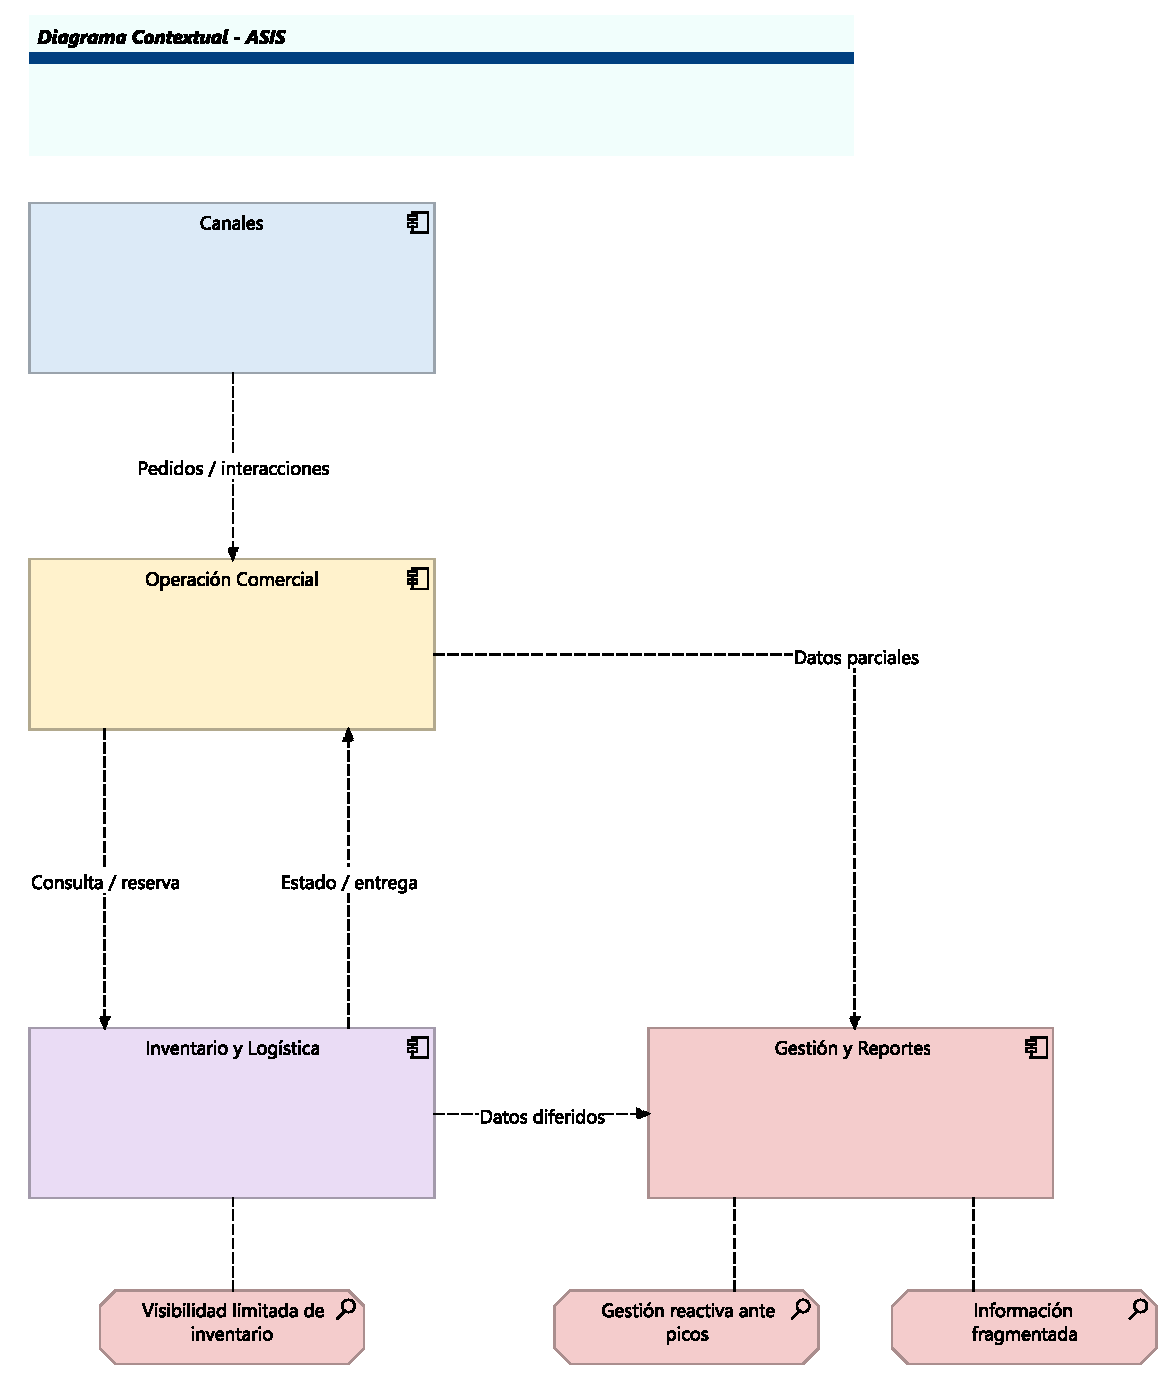
\includegraphics[width=\linewidth,height=16cm,keepaspectratio]{01_contextual_asis.pdf}
\caption{Vista contextual AS-IS de extremo a extremo}
\Fuente{Modelo de solución elaborado por el equipo~\cite{modelo-solucion}}
\end{figure}

\newcommand{\Lamina}[3]{%
\clearpage\begin{landscape}
\thispagestyle{fancy}
\subsection*{#1}
\begin{figure}[H]\centering
\includegraphics[width=.98\linewidth,height=13.0cm,keepaspectratio]{#2}
\caption{#3}\Fuente{Modelo de solución elaborado por el equipo~\cite{modelo-solucion}}
\end{figure}
\end{landscape}}
\Lamina{Contexto de la solución propuesta}{02_contextual_tobe.pdf}{Vista contextual TO-BE de extremo a extremo}
\Lamina{Proceso actual de atención}{03_pedidos_asis.pdf}{Vista completa de atención de pedidos AS-IS}
\Lamina{Proceso propuesto de atención}{04_pedidos_tobe.pdf}{Vista completa de atención inteligente de pedidos TO-BE}
\Lamina{Aplicaciones y procesos actuales}{05_aplicaciones_procesos_asis.pdf}{Relación entre aplicaciones y procesos AS-IS}
\Lamina{Aplicaciones y procesos propuestos}{06_aplicaciones_procesos_tobe.pdf}{Relación entre aplicaciones y procesos TO-BE}
\Lamina{Integración macro de la solución}{07_integracion_macro_tobe.pdf}{Vista macro de componentes e integración}

\LuminaDetalleBegin
\thispagestyle{empty}
\begin{center}
{\Large\bfseries Integración detallada de la solución\par}
\vspace{5mm}
\begin{figure}[H]
\centering
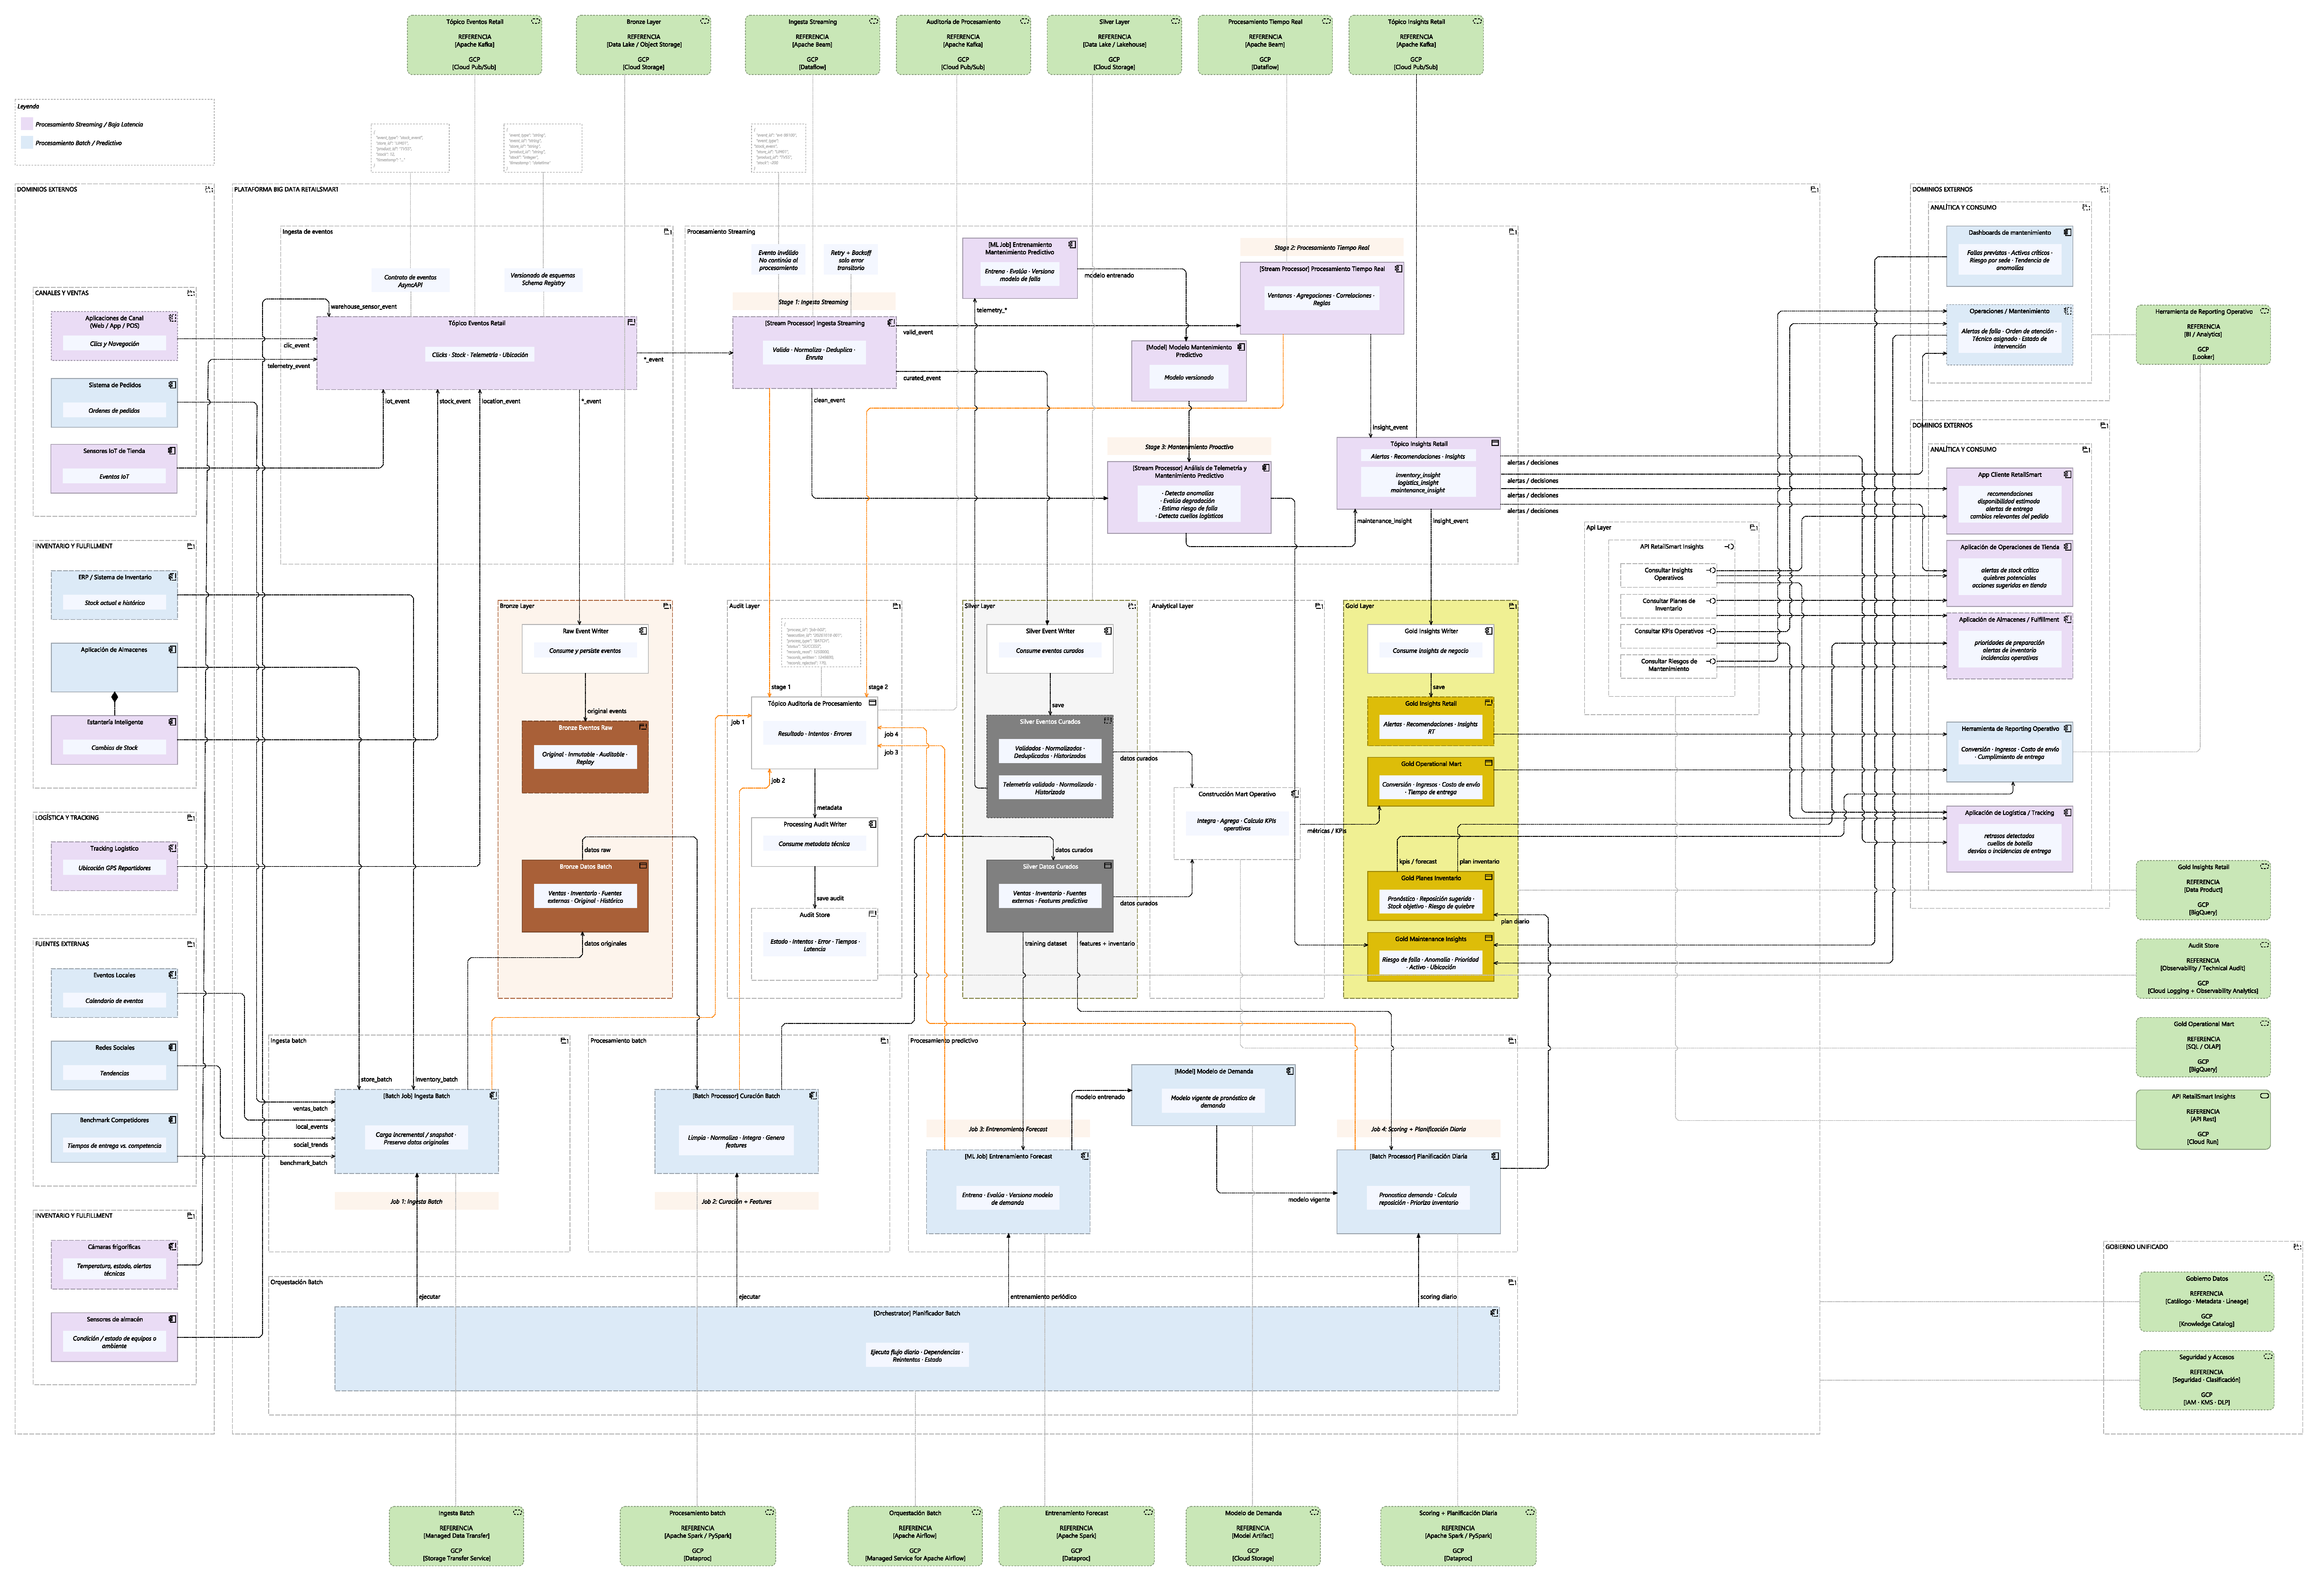
\includegraphics[
  width=\linewidth,
  height=165mm,
  keepaspectratio
]{08_integracion_detallada_tobe.pdf}
\caption{Vista detallada de componentes e integración}\label{fig:integracion-detallada}
\Fuente{Modelo de solución elaborado por el equipo~\cite{modelo-solucion}}
\end{figure}
\end{center}
\LuminaDetalleRestore
\end{document}
